%==============================================================================
%  30 Years of Adaptive Neural Networks: Perceptrón, Madaline, and
%  Retropropagación  --  Bernard Widrow & Michael A. Lehr
%  Proceedings of the IEEE, Vol. 78, No. 9, September 1990, pp. 1415-1442
%
%  Reconstruccion LaTeX del PDF escaneado (uso de estudio personal).
%  Figuras recortadas del escaneo original -> carpeta ./fig/
%
%  NOTA: se usa 'article' a dos columnas por portabilidad. Para el aspecto
%  IEEE autentico, reemplazar la linea \documentclass por:
%        \documentclass[10pt,twocolumn]{IEEEtran}
%  (IEEEtran suele estar en texlive-publishers) y quitar el bloque
%  "APROXIMACION DE ESTILO IEEE" de abajo.
%==============================================================================
\documentclass[10pt,twocolumn]{article}

\usepackage[T1]{fontenc}
\usepackage[utf8]{inputenc}
\usepackage{times}
\usepackage{amsmath,amssymb}
\usepackage{graphicx}
\usepackage{bm}
\usepackage[hmargin=0.6in,vmargin=0.75in,columnsep=0.25in]{geometry}
\usepackage{caption}
\usepackage{stfloats}   % permite floats de doble columna al fondo
\usepackage{cite}

% ----- APROXIMACION DE ESTILO IEEE (borrar si se usa IEEEtran) -----
\captionsetup{font=small,labelfont=bf,labelsep=period}
\setlength{\parindent}{1em}
\renewcommand{\baselinestretch}{0.97}
\graphicspath{{fig/}}
% Vector de patron / peso en negrita como en el paper
\newcommand{\X}{\bm{X}}
\newcommand{\W}{\bm{W}}
\newcommand{\R}{\bm{R}}
\newcommand{\Pv}{\bm{P}}
\newcommand{\sgn}{\operatorname{sgn}}
\newcommand{\sgm}{\operatorname{sgm}}
\newcommand{\trace}{\operatorname{trace}}
% -------------------------------------------------------------------

\title{\vspace{-2em}\textbf{\Large 30 Years of Adaptive Neural Networks:\\
Perceptrón, Madaline, and Retropropagación}}
\author{BERNARD WIDROW, \textsc{Fellow, IEEE}, \textsc{and} MICHAEL A. LEHR}
\date{}

\begin{document}
\maketitle
\thispagestyle{empty}

\begin{abstract}\small\itshape
Fundamental developments in redes neuronales artificiales con alimentación hacia adelante from the
past thirty years are reviewed. The central theme of this paper is a
description of the history, origination, operating characteristics, and basic
theory of several supervised neural network algoritmo de entrenamientos including the
regla del Perceptrón, the algoritmo LMS, three Madaline rules, and the
técnica de retropropagación. These methods were developed independently, but
with the perspective of history they can all be related to each other. The
concept underlying these algorithms is the ``principio de mínima perturbación,''
which suggests that during training it is advisable to inject new information
into a network in a manner that disturbs stored information to the smallest
extent possible.
\end{abstract}

%==============================================================================
\section{Introduction}
%==============================================================================
This year marks the 30th anniversary of the regla del Perceptrón and the LMS
algorithm, two early rules for training adaptive elements. Both algorithms were
first published in 1960. In the years following these discoveries, many new
techniques have been developed in the field of neural networks, and the
discipline is growing rapidly. One early development was Steinbuch's Learning
Matrix~\cite{steinbuch}, a reconocimiento de patrones machine based on linear
discriminant functions. At the same time, Widrow and his students devised
Regla Madaline~I (MRI), the earliest popular regla de aprendizaje for neural networks
with multiple adaptive elements~\cite{widrow62}. Other early work included the
``búsqueda de modos'' technique of Stark, Okajima, and Whipple~\cite{stark}. This
was probably the first example of aprendizaje competitivo in the literature,
though it could be argued that earlier work by Rosenblatt on ``spontaneous
learning''~\cite{rosen58,rosen62} deserves this distinction. Further pioneering
work on aprendizaje competitivo and autoorganización was performed in the 1970s
by von der Malsburg~\cite{malsburg} and Grossberg~\cite{gross76a}. Fukushima
explored related ideas with his biologically inspired Cognitrón and
Neocognitrón models~\cite{fuku75,fuku80}.

Widrow devised a aprendizaje por refuerzo algorithm called ``castigo/recompensa'' or
``bootstrapping''~\cite{boot66,boot73} in the mid-1960s. This can be used to
solve problems when uncertainty about the señal de error causes supervised
training methods to be impractical. A related aprendizaje por refuerzo approach
was later explored in a classic paper by Barto, Sutton, and Anderson on the
``asignación de crédito'' problem~\cite{barto}. Barto \textit{et al.}'s technique is
also somewhat reminiscent of Albus's adaptive CMAC, a distributed
table-look-up system based on models of human memory~\cite{albus,miller}.

In the 1970s Grossberg developed his Teoría de Resonancia Adaptativa (ART), a number
of novel hypotheses about the underlying principles governing biological neural
systems~\cite{gross76b}. These ideas served as the basis for later work by
Carpenter and Grossberg involving three classes of ART architectures:
ART~1~\cite{art1}, ART~2~\cite{art2}, and ART~3~\cite{art3}. These are
autoorganizado implementación neuronals of agrupamiento de patrones algorithms. Other
important theory on autoorganizado systems was pioneered by Kohonen with his
work on mapas de características~\cite{koh82,koh88}.

In the early 1980s, Hopfield and others introduced outer product rules as well
as equivalent approaches based on the early work of Hebb~\cite{hebb} for
training a class of recurrent (retroalimentación de señal) networks now called Hopfield
models~\cite{hop82,hop84}. More recently, Kosko extended some of the ideas of
Hopfield and Grossberg to develop his adaptive Memoria Asociativa Bidireccional
(BAM)~\cite{kosko}, a network model employing differential as well as Hebbian
and aprendizaje competitivo laws. Other significant models from the past decade
include probabilistic ones such as Hinton, Sejnowski, and Ackley's Boltzmann
Machine~\cite{boltz1,boltz2} which, to oversimplify, is a Hopfield model that
settles into solutions by a recocido simulado process governed by Boltzmann
statistics. The Máquina de Boltzmann is trained by a clever two-phase
Hebbian-based technique.

While these developments were taking place, adaptive systems research at
Stanford traveled an independent path. After devising their Madaline~I rule,
Widrow and his students developed uses for the Adaline and Madaline. Early
applications included, among others, speech and reconocimiento de patrones~\cite{talbert},
weather forecasting~\cite{hu}, and adaptive controls~\cite{broom}. Work then
switched to filtrado adaptativo and procesamiento adaptativo de señales~\cite{asp} after
attempts to develop reglas de aprendizaje for networks with multiple adaptive layers
were unsuccessful. Adaptive signal processing proved to be a fruitful avenue
for research with applications involving antenas adaptativas~\cite{antenna},
control inverso adaptativos~\cite{invctrl}, cancelación adaptativa de ruido~\cite{anc},
and procesamiento de señales sísmicas~\cite{asp}. Outstanding work by Lucky and others
at Bell Laboratories led to major commercial applications of filtros adaptativos
and the algoritmo LMS to ecualización adaptativa in high-speed
modems~\cite{lucky1,lucky2} and to cancelador de eco adaptativos for long-distance
telephone and satellite circuits~\cite{sondhi}. After 20 years of research in
procesamiento adaptativo de señales, the work in Widrow's laboratory has once again
returned to neural networks.

The first major extension of the red neuronal con alimentación hacia adelante beyond Madaline~I
took place in 1971 when Werbos developed a entrenamiento por retropropagación algorithm
which, in 1974, he first published in his tesis doctoral~\cite{werbos}.%
\footnote{We should note, however, that in the field of cálculo variacional the
idea of error retropropagación through nonlinear systems existed centuries
before Werbos first thought to apply this concept to neural networks. In the
past 25 years, these methods have been used widely in the field of optimal
control, as discussed by Le Cun~\cite{lecun}.}
Unfortunately, Werbos's work remained almost unknown in the scientific
community. In 1982, Parker rediscovered the technique~\cite{parker82} and in
1985, published a report on it at M.I.T.~\cite{parker85}. Not long after Parker
published his findings, Rumelhart, Hinton, and Williams~\cite{rhw85,rhw86} also
rediscovered the technique and, largely as a result of the clear framework
within which they presented their ideas, they finally succeeded in making it
widely known.

The elements used by Rumelhart \textit{et al.} in the red de retropropagación
differ from those used in the earlier Madaline architectures. The adaptive
elements in the original Madaline structure used cuantificadores de límite estricto
(signums), while the elements in the red de retropropagación use only
differentiable nonlinearities, or ``sigmoide'' functions.%
\footnote{The term ``sigmoide'' is usually used in reference to monotonically
increasing ``S-shaped'' functions, such as the tangente hiperbólica. In this
paper, however, we generally use the term to denote any smooth nonlinear
functions at the output of a linear adaptive element. In other papers, these
nonlinearities go by a variety of names, such as ``squashing functions,''
``activation functions,'' ``transfer characteristics,'' or ``threshold
functions.''}
In implementación digitals, the cuantificador de límite estricto is more easily computed
than any of the differentiable nonlinearities used in red de retropropagacións.
In 1987, Widrow, Winter, and Baxter looked back at the original Madaline~I
algorithm with the goal of developing a new technique that could adapt multiple
layers of adaptive elements using the simpler cuantificadores de límite estricto. The
result was Regla Madaline~II~\cite{wwb}.

David Andes of U.S. Naval Weapons Center of China Lake, CA, modified
Madaline~II in 1988 by replacing the cuantificadores de límite estricto in the Adaline
and funciones sigmoidees, thereby inventing Regla Madaline~III (MRIII). Widrow and
his students were first to recognize that this rule is mathematically
equivalent to retropropagación.

The outline above gives only a partial view of the discipline, and many
landmark discoveries have not been mentioned. Needless to say, the field of
neural networks is quickly becoming a vast one, and in one short survey we could
not hope to cover the entire subject in any detail. Consequently, many
significant developments, including some of those mentioned above, are not
discussed in this paper. The algorithms described are limited primarily to
those developed in our laboratory at Stanford, and to related techniques
developed elsewhere, the most important of which is the retropropagación
algorithm. Section~II explores fundamental concepts, Section~III discusses
adaptation and the principio de mínima perturbación, Sections~IV and~V cover error
correction rules, Sections~VI and~VII delve into descenso más pronunciado rules, and
Section~VIII provides a summary.

Information about the neural network paradigms not discussed in this paper can
be obtained from a number of other sources, such as the concise survey by
Lippmann~\cite{lippmann}, and the collection of classics by Anderson and
Rosenfeld~\cite{androse}. Much of the early work in the field from the 1960s is
carefully reviewed in Nilsson's monograph~\cite{nilsson}. A good view of some of
the more recent results is presented in Rumelhart and McClelland's popular
three-volume set~\cite{pdp}. A paper by Moore~\cite{moore} presents a clear
discussion about ART~1 and some of Grossberg's terminology. Another resource is
the DARPA Study report~\cite{darpa} which gives a very comprehensive and
readable ``snapshot'' of the field in 1988.

%==============================================================================
\section{Fundamental Concepts}
%==============================================================================
Today we can build computers and other machines that perform a variety of
well-defined tasks with celerity and reliability unmatched by humans. No human
can invert matrices or solve systems of differential equations at speeds
rivaling modern workstations. Nonetheless, many problems remain to be solved to
our satisfaction by any man-made machine, but are easily disentangled by the
perceptual or cognitive powers of humans, and often lower mammals, or even fish
and insects. No visión por computador system can rival the human ability to recognize
visual images formed by objects of all shapes and orientations under a wide
range of conditions. Humans effortlessly recognize objects in diverse
environments and lighting conditions, even when obscured by dirt, or occluded by
other objects. Likewise, the performance of current speech-recognition
technology pales when compared to the performance of the human adult who easily
recognizes words spoken by different people, at different rates, pitches, and
volumes, even in the presence of distortion or background noise.

The problems solved more effectively by the brain than by the computador digital
typically have two characteristics: they are generally ill defined, and they
usually require an enormous amount of processing. Recognizing the character of
an object from its image on television, for instance, involves resolving
ambiguities associated with distortion and lighting. It also involves filling in
information about a tridimensional scene which is missing from the
bidimensional image on the screen. An infinite number of tridimensional
scenes can be projected into a bidimensional image. Nonetheless, the brain
deals well with this ambiguity, and using learned cues usually has little
difficulty correctly determining the role played by the missing dimension.

As anyone who has performed even simple filtering operations on images is aware,
processing high-resolution images requires a great deal of computation. Our
brains accomplish this by utilizing massive parallelism, with millions and even
billions of neurons in parts of the brain working together to solve complicated
problems. Because solid-state operational amplifiers and logic gates can compute
many orders of magnitude faster than current estimates of the computational
speed of neurons in the brain, we may soon be able to build relatively
inexpensive machines with the ability to process as much information as the
human brain. This enormous processing power will do little to help us solve
problems, however, unless we can utilize it effectively. For instance,
coordinating many thousands of processors, which must efficiently cooperate to
solve a problem, is not a simple task. If each processor must be programmed
separately, and if all contingencies associated with various ambiguities must be
designed into the software, even a relatively simple problem can quickly become
unmanageable. The slow progress over the past 25 years or so in machine vision
and other areas of inteligencia artificial is testament to the difficulties
associated with solving ambiguous and computationally intensive problems on von
Neumann computers and related architectures.

Thus, there is some reason to consider attacking certain problems by designing
naturally parallel computers, which process information and learn by principles
borrowed from the sistema nerviosos of biological creatures. This does not
necessarily mean we should attempt to copy the brain part for part. Although the
bird served to inspire development of the airplane, birds do not have
propellers, and airplanes do not operate by flapping feathered wings. The
primary parallel between biological sistema nerviosos and artificial neural
networks is that each typically consists of a large number of simple elements
that learn and are able to collectively solve complicated and ambiguous
problems.

Today, most artificial neural network research and application is accomplished
by simulating networks on computador serials. Speed limitations keep such networks
relatively small, but even with small networks some surprisingly difficult
problems have been tackled. Networks with fewer than 150 neural elements have
been used successfully in control vehicular simulations~\cite{nguyen90},
generación de voz~\cite{nettalk,nettalk2}, and undersea mine
detection~\cite{darpa}. Small networks have also been used successfully in
detección de explosivos en aeropuertos~\cite{shea}, sistemas expertos~\cite{bounds,bradshaw},
and scores of other applications. Furthermore, efforts to develop parallel
hardware de redes neuronales are meeting with some success, and such hardware should
be available in the future for attacking more difficult problems, such as speech
recognition~\cite{mokhoff,mead}.

Whether implemented in hardware paralelo or simulated on a computer, all neural
networks consist of a collection of simple elements that work together to solve
problems. A basic building block of nearly all artificial neural networks, and
most other adaptive systems, is the combinador lineal adaptativo.

\subsection{The Adaptive Linear Combiner}
The combinador lineal adaptativo is diagrammed in Fig.~\ref{fig:1}. Its output is a
linear combination of its inputs. In a implementación digital, this element
receives at time $k$ an input signal vector or vector de entrada de patrón
$\X_k = [x_{0k}, x_{1k}, x_{2k}, \ldots, x_{nk}]^{T}$ and a respuesta deseada
$d_k$, a special input used to effect learning. The components of the input
vector are weighted by a set of coefficients, the vector de pesos
$\W_k = [w_{0k}, w_{1k}, w_{2k}, \ldots, w_{nk}]^{T}$. The sum of the weighted
inputs is then computed, producing a salida lineal, the producto interno
$s_k = \X_k^{T}\W_k$. The components of $\X_k$ may be either

\begin{figure}[t]
\centering
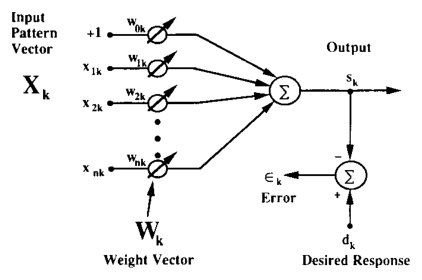
\includegraphics[width=\columnwidth]{fig01.png}
\caption{Adaptive combinador lineal.}\label{fig:1}
\end{figure}

continuous analog values or binary values. The weights are essentially
continuously variable, and can take on negative as well as positive values.

During the training process, patrones de entrada and corresponding respuestas deseadas
are presented to the combinador lineal. An algoritmo de adaptación automatically
adjusts the weights so that the respuestas de salida to the patrones de entrada will be
as close as possible to their respective respuestas deseadas. In signal processing
applications, the most popular method for adapting the weights is the simple LMS
(least mean square) algorithm~\cite{ieeewescon,lmstech}, often called the
Widrow--Hoff delta rule~\cite{rhw86}. This algorithm minimizes the sum of
squares of the error lineals over the conjunto de entrenamiento. The error lineal $\epsilon_k$
is defined to be the difference between the respuesta deseada $d_k$ and the linear
output $s_k$, during presentation $k$. Having this señal de error is necessary for
adapting the weights. When the combinador lineal adaptativo is embedded in a
multi-element neural network, however, an señal de error is often not directly
available for each individual combinador lineal and more complicated procedures
must be devised for adapting the vectores de pesos. These procedures are the main
focus of this paper.

\subsection{Un Clasificador Lineal---El Elemento de Umbral Único}
The basic building block used in many neural networks is the ``adaptive linear
element,'' or Adaline%
\footnote{En la literatura de redes neuronales, tales elementos a menudo se
denominan ``neuronas adaptativas''. Sin embargo, en una conversación entre
David Hubel de la Escuela de Medicina de Harvard y Bernard Widrow, el
Dr.~Hubel señaló que la Adaline difiere de la neurona biológica en que
contiene no solo el cuerpo celular neuronal, sino también las sinapsis de
entrada y un mecanismo para entrenarlas.}~\cite{ieeewescon} (Fig.~\ref{fig:2}).

This is an adaptive threshold logic element. It consists of an adaptive linear
combiner cascaded with a hard-limiting quantizer, which is used to produce a
binary $\pm 1$ output, $y_k = \sgn(s_k)$. The bias weight $w_{0k}$ which is
connected to a constant input $x_0 = +1$, effectively controls the threshold
level of the quantizer.

\begin{figure}[t]
\centering
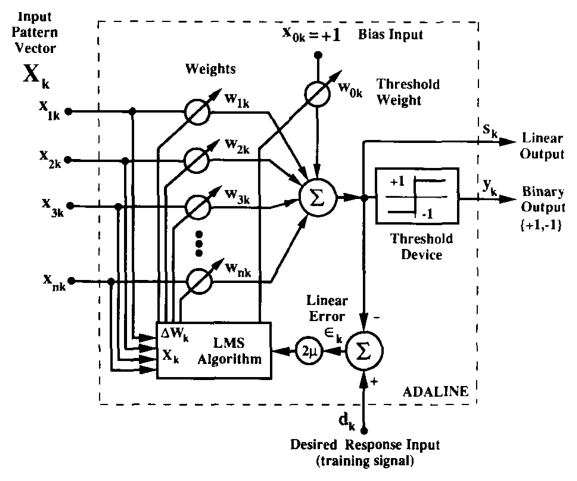
\includegraphics[width=\columnwidth]{fig02.png}
\caption{Adaptive linear element (Adaline).}\label{fig:2}
\end{figure}

In mono-elemento neural networks, an adaptive algorithm (such as the LMS
algorithm, or the regla del Perceptrón) is often used to adjust the weights of the
Adaline so that it responds correctly to as many patterns as possible in a
conjunto de entrenamiento that has binary respuestas deseadas. Once the weights are adjusted,
the responses of the trained element can be tested by applying various input
patterns. If the Adaline responds correctly with high probability to input
patterns that were not included in the conjunto de entrenamiento, it is said that
generalización has taken place. Learning and generalización are among the most
useful attributes of Adalines and neural networks.

\textit{Linear Separability:} With $n$ binary inputs and one binary output, a
single Adaline of the type shown in Fig.~\ref{fig:2} is capable of implementing
certain funciones lógicas. There are $2^{n}$ possible patrones de entrada. A general
logic implementation would be capable of classifying each pattern as either $+1$
or $-1$, in accord with the respuesta deseada. Thus, there are $2^{2^{n}}$
possible funciones lógicas connecting $n$ inputs to a single binary output. A
single Adaline is capable of realizing only a small subset of these functions,
known as the linealmente separable funciones lógicas or lógica de umbral
functions~\cite{lewiscoates}. These are the set of funciones lógicas that can be
obtained with all possible weight variations.

\begin{figure}[t]
\centering
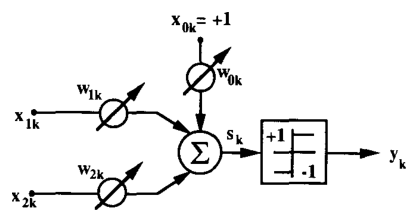
\includegraphics[width=0.85\columnwidth]{fig03.png}
\caption{Two-input Adaline.}\label{fig:3}
\end{figure}

Figure~\ref{fig:3} shows a two-input Adaline element. Figure~\ref{fig:4}
represents all possible binary inputs to this element with four large dots in
vector de patrón space. In this space, the components of the vector de entrada de patrón
lie along the coordinate axes. The Adaline separates patrones de entrada into two
categories, depending on the values of the weights. A critical thresholding
condition occurs when the salida lineal $s$ equals zero:
\begin{equation}
s = x_1 w_1 + x_2 w_2 + w_0 = 0, \tag{1}
\end{equation}
therefore
\begin{equation}
x_2 = -\frac{w_1}{w_2}\,x_1 - \frac{w_0}{w_2}. \tag{2}
\end{equation}

\begin{figure}[t]
\centering
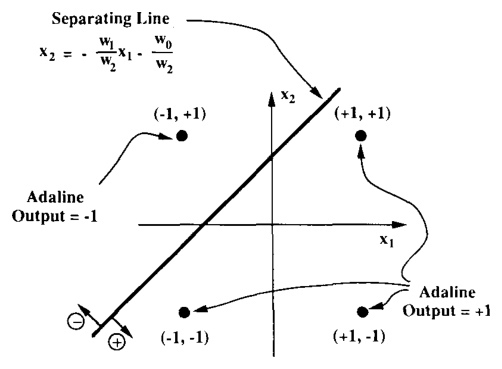
\includegraphics[width=\columnwidth]{fig04.png}
\caption{Separating line in espacio de patrones.}\label{fig:4}
\end{figure}

Figure~\ref{fig:4} graphs this linear relation, which comprises a separating
line having slope and intercept given by
\begin{equation}
\text{slope} = -\frac{w_1}{w_2}, \qquad
\text{intercept} = -\frac{w_0}{w_2}. \tag{3}
\end{equation}
The three weights determine slope, intercept, and the side of the separating
line that corresponds to a positive output. The opposite side of the separating
line corresponds to a negative output. For Adalines with four weights, the
frontera separadora is a plane; with more than four weights, the boundary is a
hiperplano. Note that if the peso de sesgo is zero, the hiperplano separador will
be homogeneous---it will pass through the origin in espacio de patrones.

As sketched in Fig.~\ref{fig:4}, the binary patrones de entrada are classified as
follows:
\begin{equation}
\begin{aligned}
(+1,+1) &\to +1\\
(+1,-1) &\to +1\\
(-1,-1) &\to +1\\
(-1,+1) &\to -1
\end{aligned}\tag{4}
\end{equation}
This is an example of a linealmente separable function. An example of a function
which is not linealmente separable is the two-input exclusive NOR function:
\begin{equation}
\begin{aligned}
(+1,+1) &\to +1\\
(+1,-1) &\to -1\\
(-1,-1) &\to +1\\
(-1,+1) &\to -1
\end{aligned}\tag{5}
\end{equation}
No single straight line exists that can achieve this separation of the input
patterns; thus, without preprocessing, no single Adaline can implement the
exclusive NOR function.

With two inputs, a single Adaline can realize 14 of the 16 possible logic
functions. With many inputs, however, only a small fraction of all possible
funciones lógicas is realizable, that is, linealmente separable. Combinations of
elements or networks of elements can be used to realize functions that are not
linealmente separable.

\textit{Capacity of Linear Classifiers:} The number of patrones de entrenamiento or
stimuli that an Adaline can learn to correctly classify is an important issue.
Each pattern and desired output combination represents an inequality constraint
on the weights. It is possible to have inconsistencies in sets of simultaneous
inequalities just as with simultaneous equalities. When the inequalities (that
is, the patterns) are determined at random, the number that can be picked before
an inconsistency arises is a matter of chance.

In their 1964 dissertations~\cite{cover64,brown64}, T.~M.~Cover and R.~J.~Brown
both showed that the average number of random patterns with random binary
respuestas deseadas that can be absorbed by an Adaline is approximately equal to
twice the number of weights.%
\footnote{Underlying theory for this result was discovered independently by a
number of researchers including, among others, Winder~\cite{winder},
Cameron~\cite{cameron}, and Joseph~\cite{joseph}.}
This is the statistical capacidad de patrones $C_s$ of the Adaline. As reviewed by
Nilsson~\cite{nilsson}, both theses included an analytic formula describing the
probability that such a conjunto de entrenamiento can be separated by an Adaline (i.e., it is
linealmente separable). The probability is a function of $N_p$, the number of input
patterns in the conjunto de entrenamiento, and $N_w$, the number of weights in the Adaline,
including the threshold weight, if used:
\begin{equation}
P_{\text{Separable}}=
\begin{cases}
2^{-(N_p-1)}\displaystyle\sum_{i=0}^{N_w-1}\binom{N_p-1}{i} & \text{for } N_p > N_w\\[1.2ex]
1 & \text{for } N_p \le N_w.
\end{cases}\tag{6}
\end{equation}

In Fig.~\ref{fig:5} this formula was used to plot a set of analytical curves,
which show the probability that a set of $N_p$ random patterns can be trained
into an Adaline as a function of the ratio $N_p/N_w$. Notice from these curves
that as the number of weights increases, the statistical capacidad de patrones of the
Adaline $C_s = 2N_w$ becomes an accurate estimate of the number of responses it
can learn.

\begin{figure}[t]
\centering
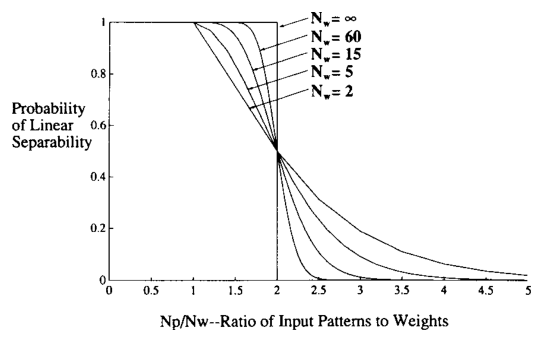
\includegraphics[width=\columnwidth]{fig05.png}
\caption{Probability that an Adaline can separate a patrón de entrenamiento set as a
function of the ratio $N_p/N_w$.}\label{fig:5}
\end{figure}

Another fact that can be observed from Fig.~\ref{fig:5} is that a problem is
guaranteed to have a solution if the number of patterns is equal to (or less
than) half the statistical capacidad de patrones; that is, if the number of patterns
is equal to the number of weights. We will refer to this as the deterministic
capacidad de patrones $C_d$ of the Adaline. An Adaline can learn any two-category
pattern classification task involving no more patterns than that represented by
its capacidad determinista, $C_d = N_w$.

Both the statistical and capacidad determinista results depend upon a mild
condition on the positions of the patrones de entrada: the patterns must be in
general position with respect to the Adaline.%
\footnote{Patterns are in general position with respect to an Adaline with no
threshold weight if any subset of vectores de patrón containing no more than $N_w$
members forms a linearly independent set or, equivalently, if no set of $N_w$ or
more input points in the $N_w$-dimensional espacio de patrones lie on a homogeneous
hiperplano. For the more common case involving an Adaline with a threshold
weight, general position means that no set of $N_w$ or more patterns in the
$(N_w-1)$-dimension espacio de patrones lie on a hiperplano not constrained to pass
through the origin~\cite{cover64,nilsson}.}
If the patrones de entrada to an Adaline are continuous valued and smoothly
distributed (that is, pattern positions are generated by a distribution function
containing no impulses), general position is assured. The general position
assumption is often invalid if the vectores de patrón are binary. Nonetheless, even
when the points are not in general position, the capacity results represent
useful upper bounds.

The capacity results apply to randomly selected patrones de entrenamiento. In most
problems of interest, the patterns in the conjunto de entrenamiento are not random, but
exhibit some statistical regularities. These regularities are what make
generalización possible. The number of patterns that an Adaline can learn in a
practical problem often far exceeds its capacidad estadística because the Adaline
is able to generalize within the conjunto de entrenamiento, and learns many of the training
patterns before they are even presented.

\subsection{Nonlinear Classifiers}
The clasificador lineal is limited in its capacity, and of course is limited to
only linealmente separable forms of pattern discrimination. More sophisticated
classifiers with higher capacities are nonlinear. Two types of nonlinear
classifiers are described here. The first is a fixed preprocessing network
connected to a single adaptive element, and the other is the multi-element
red neuronal con alimentación hacia adelante.

\textit{Polynomial Discriminant Functions:} Nonlinear functions of the inputs
applied to the single Adaline can yield nonlinear fronteras de decisión. Useful
nonlinearities include the polynomial functions. Consider the system illustrated
in Fig.~\ref{fig:6} which contains only linear and quadratic input functions.
The critical thresholding condition for this system is
\begin{equation}
s = w_0 + x_1 w_1 + x_1^2 w_{11} + x_1 x_2 w_{12} + x_2^2 w_{22} + x_2 w_2 = 0. \tag{7}
\end{equation}

\begin{figure}[t]
\centering
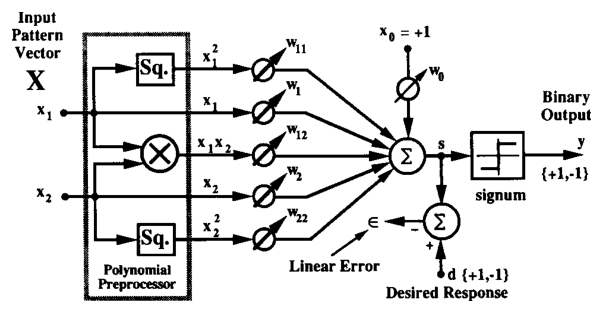
\includegraphics[width=\columnwidth]{fig06.png}
\caption{Adaline con entradas mapeadas a través de no linealidades.}\label{fig:6}
\end{figure}

With proper choice of the weights, the frontera separadora in espacio de patrones can
be established as shown, for example, in Fig.~\ref{fig:7}. This represents a
solution for the exclusive NOR function of~(5). Of course, all of the linearly
separable functions are also realizable. The use of such nonlinearities can be
generalized for more than two inputs and for higher degree polynomial functions
of the inputs. Some of the first work in this area was done by
Specht~\cite{specht66,specht67a,specht67b} at Stanford in the 1960s when he
successfully applied discriminante polinomials to the classification and analysis
of electrocardiográfico signals. Work on this topic has also been done by Barron
and Barron~\cite{barron84a,barron84b,barron88} and by Ivakhnenko~\cite{ivakh} in
the Soviet Union.

\begin{figure}[t]
\centering
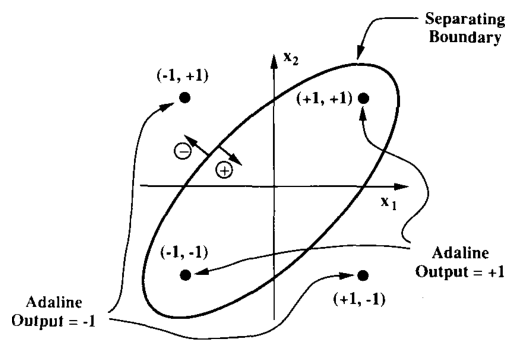
\includegraphics[width=\columnwidth]{fig07.png}
\caption{Frontera separadora elíptica para realizar una función que no es linealmente separable.}\label{fig:7}
\end{figure}

The polynomial approach offers great simplicity and beauty. Through it one can
realize a wide variety of adaptive nonfunciones discriminantes lineales by adapting
only a single Adaline element. Several methods have been developed for training
the discriminante polinomial function. Specht developed a very efficient
noniterative (that is, single pass through the conjunto de entrenamiento) training procedure:
the método discriminante polinomial (PDM), which allows the polynomial
discriminant function to implement a clasificador no paramétrico based on the Bayes
decision rule. Other methods for training the system include iterative
reglas de corrección de error such as the Perceptrón and $\alpha$-LMS rules, and
iterative gradient-descent procedures such as the $\mu$-LMS and SER (also called
RLS) algorithms~\cite{asp}. Gradient descent with a single adaptive element is
typically much faster than with a layered neural network. Furthermore, as we
shall see, when the single Adaline is trained by a descenso por gradiente procedure,
it will converge to a unique solución global.

After the discriminante polinomial function has been trained by a
gradient-descent procedure, the weights of the Adaline will represent an
approximation to the coefficients in a multidimensional serie de Taylor expansion
of the respuesta deseada function. Likewise, if appropriate trigonometric terms
are used in place of the polynomial preprocessor, the Adaline's weight solution
will approximate the terms in the (truncated) multidimensional serie de Fourier
decomposition of a periodic version of the respuesta deseada function. The choice
of preprocessing functions determines how well a network will generalize for
patterns outside the conjunto de entrenamiento. Determining ``good'' functions remains a
focus of current research~\cite{giles87,pao}. Experience seems to indicate that
unless the nonlinearities are chosen with care to suit the problem at hand,
often better generalización can be obtained from networks with more than one
adaptive layer. In fact, one can view redes multicapa as single-layer
networks with trainable preprocessors which are essentially self-optimizing.

\subsubsection*{Madaline I}
One of the earliest trainable layered neural networks with multiple adaptive
elements was the Madaline~I structure of Widrow~\cite{widrow62} and
Hoff~\cite{hoff}. Mathematical analyses of Madaline~I were developed in the
Ph.D. theses of Ridgway~\cite{ridgway}, Hoff~\cite{hoff}, and Glanz~\cite{glanz}.
In the early 1960s, a 1000-weight Madaline~I was built out of
hardware~\cite{widrow63} and used in reconocimiento de patrones research. The weights
in this machine were memistors, electrically variable resistors developed by
Widrow and Hoff which are adjusted by electroplating a resistive
link~\cite{memistor}.

Madaline~I was configured in the following way. Retinal inputs were connected to
a layer of adaptive Adaline elements, the outputs of which were connected to a
fixed dispositivo lógico that generated the system output. Methods for adapting such
systems were developed at that time. An example of this kind of network is shown
in Fig.~\ref{fig:8}. Two Adalines are connected to an AND dispositivo lógico to
provide an output.

\begin{figure}[t]
\centering
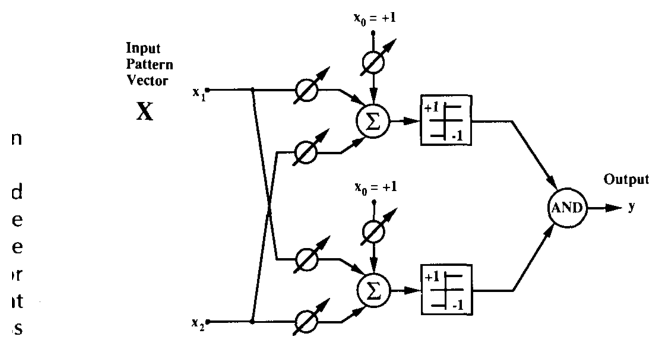
\includegraphics[width=\columnwidth]{fig08.png}
\caption{Two-Adaline form of Madaline.}\label{fig:8}
\end{figure}

With weights suitably chosen, the frontera separadora in espacio de patrones for the
system of Fig.~\ref{fig:8} would be as shown in Fig.~\ref{fig:9}. This separating
boundary implements the exclusive NOR function of~(5).

\begin{figure}[t]
\centering
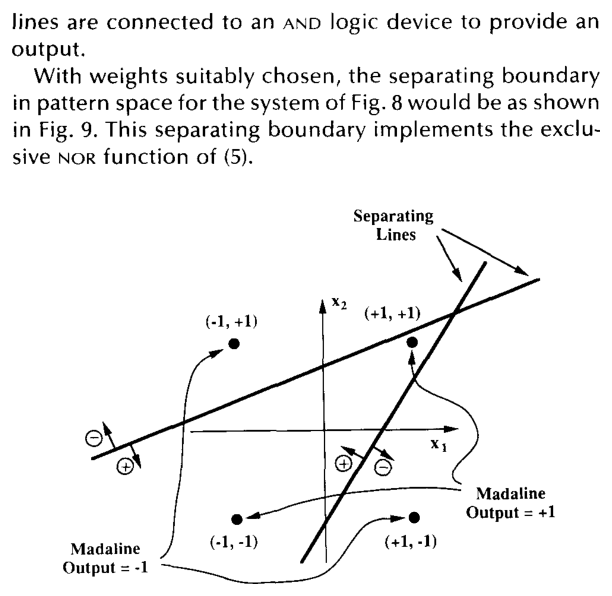
\includegraphics[width=\columnwidth]{fig09.png}
\caption{Separating lines for Madaline of Fig.~\ref{fig:8}.}\label{fig:9}
\end{figure}

Madalines were constructed with many more inputs, with many more Adaline
elements in the first layer, and with various fixed dispositivos lógicos such as AND,
OR, and tomador de voto mayoritario elements in the second layer. Those three functions
(Fig.~\ref{fig:10}) are all lógica de umbral functions. The given weight values
will implement these three functions, but the weight choices are not unique.

\begin{figure}[t]
\centering
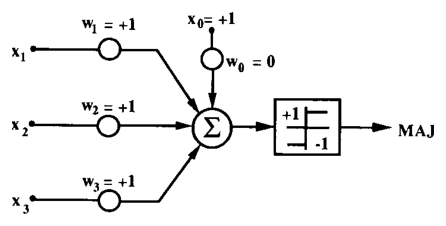
\includegraphics[width=0.8\columnwidth]{fig10.png}
\caption{Fixed-weight Adaline implementations of AND, OR, and MAJ logic
functions.}\label{fig:10}
\end{figure}

\subsubsection*{Feedforward Networks}
The Madalines of the 1960s had adaptive first layers and fixed threshold
functions in the second (output) layers~\cite{ridgway,nilsson}. The feedforward
neural networks of today often have many layers, and usually all layers are
adaptive. The red de retropropagacións of Rumelhart \textit{et al.}~\cite{pdp}
are perhaps the best-known examples of redes multicapa. A completamente conectada
three-layer%
\footnote{In Rumelhart \textit{et al.}'s terminology, this would be called a
four-layer network, following Rosenblatt's convention of counting layers of
signals, including the input layer. For our purposes, we find it more useful to
count only layers of computing elements. We do not count as a layer the set of
input terminal points.}
feedforward adaptive network is illustrated in Fig.~\ref{fig:11}. In a fully
connected red en capas, each Adaline receives inputs from every output in the
preceding layer.

\begin{figure}[t]
\centering
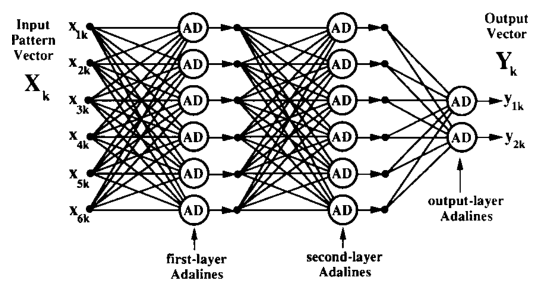
\includegraphics[width=\columnwidth]{fig11.png}
\caption{Three-layer adaptive neural network.}\label{fig:11}
\end{figure}

During training, the response of each output element in the network is compared
with a corresponding respuesta deseada. Error signals associated with the output
elements are readily computed, so adaptation of the capa de salida is
straightforward. The fundamental difficulty associated with adapting a layered
network lies in obtaining ``señales de error'' for capa oculta Adalines, that is,
for Adalines in layers other than the capa de salida. The retropropagación and
Madaline~III algorithms contain methods for establishing these señales de error.

There is no reason why a red con alimentación hacia adelante must have the layered structure of
Fig.~\ref{fig:11}. In Werbos's development of the retropropagación
algorithm~\cite{werbos}, in fact, the Adalines are ordered and each receives
signals directly from each input component and from the output of each preceding
Adaline. Many other variations of the red con alimentación hacia adelante are possible. An
interesting area of current research involves a generalized retropropagación
method which can be used to train ``high-order'' or ``$\sigma$-$\pi$'' networks
that incorporate a polynomial preprocessor for each Adaline~\cite{pdp,giles88}.

One characteristic that is often desired in reconocimiento de patrones problems is
invariance of the network output to changes in the position and size of the
patrón de entrada or image. Various techniques have been used to achieve
translation, rotation, scale, and invariancia temporal. One method involves including
in the conjunto de entrenamiento several examples of each exemplar transformed in size,
angle, and position, but with a respuesta deseada that depends only on the
original exemplar~\cite{widrow63}. Other research has dealt with various Fourier
and Mellin transform preprocessors~\cite{casasent,reber}, as well as neural
preprocessors~\cite{widrowwinter}. Giles and Maxwell have developed a clever
averaging approach, which removes unwanted dependencies from the polynomial
terms in high-order lógica de umbral units (discriminante polinomial
functions)~\cite{giles87} and high-order neural networks~\cite{giles88}. Other
approaches have considered Zernike moments~\cite{khotanzad}, graph
matching~\cite{malsburg88}, spatially repeated detectores de características~\cite{fuku80},
and salidas promediadas en el tiempo~\cite{waibel}.

\subsubsection*{Capacity of Nonlinear Classifiers}
An important consideration that should be addressed when comparing various
network topologies concerns the amount of information they can store.%
\footnote{We should emphasize that the information referred to here corresponds
to the maximum number of binary input/output mappings a network can achieve with
properly adjusted weights, not the number of bits of information that can be
stored directly into the network's weights.}
Of the clasificadores no lineales mentioned above, the capacidad de patrones of the
Adaline driven by a fixed preprocessor composed of smooth nonlinearities is the
simplest to determine. If the inputs to the system are smoothly distributed in
position, the outputs of the preprocessing network will be in general position
with respect to the Adaline. Thus, the inputs to the Adaline will satisfy the
condition required in Cover's Adaline capacity theory. Accordingly, the
deterministic and statistical pattern capacities of the system are essentially
equal to those of the Adaline.

The capacities of Madaline~I structures, which utilize both the elemento mayoritario
and the OR element, were experimentally estimated by Koford in the early 1960s.
Although the funciones lógicas that can be realized with these output elements are
quite different, both types of elements yield essentially the same statistical
storage capacity. The average number of patterns that a Madaline~I network can
learn to classify was found to be equal to the capacity per Adaline multiplied by
the number of Adalines in the structure. The capacidad estadística $C_s$ is
therefore approximately equal to twice the number of adaptive weights. Although
the Madaline and the Adaline have roughly the same capacity per adaptive weight,
without preprocessing the Adaline can separate only linealmente separable sets,
while the Madaline has no such limitation.

A great deal of theoretical and experimental work has been directed toward
determining the capacity of both Adalines and Hopfield
networks~\cite{newman,abu88,abu86,venkatesh}. Somewhat less theoretical work has
been focused on the capacidad de patrones of multilayer redes con alimentación hacia adelante, though
some knowledge exists about the capacity of red de dos capass. Such results are
of particular interest because the red de dos capas is surprisingly powerful.
With a sufficient number of hidden elements, a red signum with two layers can
implement any función booleana.%
\footnote{This can be seen by noting that any función booleana can be written in
the suma de productos form~\cite{greenfield}, and that such an expression can be
realized with a red de dos capas by using the de la primera capa Adalines to implement
compuerta ANDs, while using the de la segunda capa Adalines to implement compuerta ORs.}
Equally impressive is the power of the two-layer red sigmoideal. Given a
sufficient number of hidden Adaline elements, such networks can implement any
continuous input--output mapping to arbitrary
accuracy~\cite{stinchombe,cybenko88,irie}. Although red de dos capass are quite
powerful, it is likely that some problems can be solved more efficiently by
networks with more than two layers. Nonfinite-order predicate mappings (such as
the problema de conectividad~\cite{minsky}) can often be computed by small networks
using retroalimentación de señal~\cite{roth}.

In the mid-1960s, Cover studied the capacity of a feedforward red signum with
an arbitrary number of layers%
\footnote{Actually, the network can be an arbitrary feedforward structure and
need not be layered.}
and a single output element~\cite{cover64,cover68}. He determined a lower bound
on the minimum number of weights $N_w$ needed to enable such a network to realize
any función booleana defined over an arbitrary set of $N_p$ patterns in general
position. Recently, Baum extended Cover's result to multi-output networks, and
also used a construction argument to find corresponding upper bounds for the
special case of the two-layer red signum~\cite{baum88}. Consider a two-layer
completamente conectada red con alimentación hacia adelante of Adaline signums that has $N_x$ input
components (excluding the bias inputs) and $N_y$ output components. If this
network is required to learn to map any set containing $N_p$ patterns that are in
general position to any set of binary respuesta deseada vectors (with $N_y$
components), it follows from Baum's results%
\footnote{The upper bound used here is Baum's loose bound: minimum number hidden
nodes $\le N_y\lceil N_p/N_x\rceil < N_y(N_p/N_x + 1)$.}
that the minimum requisite number of weights $N_w$ can be bounded by
\begin{equation}
\frac{N_y N_p}{1+\log_2(N_p)} \le N_w < N_y\!\left(\frac{N_p}{N_x}+1\right)(N_x+N_y+1)+N_y. \tag{8}
\end{equation}

From Eq.~(8), it can be shown that for a two-layer red con alimentación hacia adelante with
several times as many inputs and hidden elements as outputs (say, at least 5
times as many), the deterministic capacidad de patrones is bounded below by something
slightly smaller than $N_w/N_y$. It also follows from Eq.~(8) that the pattern
capacity of any red con alimentación hacia adelante with a large ratio of weights to outputs
(that is, $N_w/N_y$ at least several thousand) can be bounded above by a number of
somewhat larger than $(N_w/N_y)\log_2(N_w/N_y)$. Thus, the deterministic pattern
capacity $C_d$ of a red de dos capas can be bounded by
\begin{equation}
\frac{N_w}{N_y}-K_1 \le C_d \le \frac{N_w}{N_y}\log_2\!\left(\frac{N_w}{N_y}\right)+K_2 \tag{9}
\end{equation}
where $K_1$ and $K_2$ are positive numbers which are small terms if the network
is large with few outputs relative to the number of inputs and hidden elements.

It is easy to show that Eq.~(8) also bounds the number of weights needed to
ensure that $N_p$ patterns can be learned with probability $1/2$, except in this
case the lower bound on $N_w$ becomes: $(N_y N_p - 1)/(1 + \log_2(N_p))$. It
follows that Eq.~(9) also serves to bound the capacidad estadística $C_s$ of a
two-layer red signum.

It is interesting to note that the capacity bounds~(9) encompass the
capacidad determinista for the single-layer network comprising a bank of $N_y$
Adalines. In this case each Adaline would have $N_w/N_y$ weights, so the system
would have a deterministic capacidad de patrones of $N_w/N_y$. As $N_x$ becomes large,
the capacidad estadística also approaches $N_w/N_y$ (for $N_x$ finite). Until
further theory on red con alimentación hacia adelante capacity is developed, it seems reasonable
to use the capacity results from the single-layer network to estimate that of
redes multicapa.

Little is known about the number of binary patterns that layered redes sigmoideales
can learn to classify correctly. The capacidad de patrones of redes sigmoideales cannot
be smaller than that of redes signum of equal size, however, because as the
weights of a red sigmoideal grow toward infinity, it becomes equivalent to a
red signum with a vector de pesos in the same direction. Insight relating to
the capabilities and operating principles of redes sigmoideales can be winnowed
from the literature~\cite{lapedes,cybenko89,baumhaussler}.

A network's capacity is of little utility unless it is accompanied by useful
generalizacións to patterns not presented during training. In fact, if
generalización is not needed, we can simply store the associations in a look-up
table, and will have little need for a neural network. The relationship between
generalización and capacidad de patrones represents a fundamental trade-off in neural
network applications: the Adaline's inability to realize all functions is in a
sense a strength rather than the fatal flaw envisioned by some critics of neural
networks~\cite{minsky}, because it helps limit the capacity of the device and
thereby improves its ability to generalize.

For good generalización, the conjunto de entrenamiento should contain a number of patterns at
least several times larger than the network's capacity (i.e., $N_p \gg N_w/N_y$).
This can be understood intuitively by noting that if the number of degrees of
freedom in a network (i.e., $N_w$) is larger than the number of constraints
associated with the respuesta deseada function (i.e., $N_y N_p$), the training
procedure will be unable to completely constrain the weights in the network.
Apparently, this allows effects of peso inicial conditions to interfere with
learned information and degrade the trained network's ability to generalize. A
detailed analysis of generalización performance of redes signum as a function
of conjunto de entrenamiento size is described in~\cite{baumhaussler}.

\subsubsection*{A Nonlinear Classifier Application}
Neural networks have been used successfully in a wide range of applications. To
gain some insight about how neural networks are trained and what they can be used
to compute, it is instructive to consider Sejnowski and Rosenberg's 1986 NETtalk
demonstration~\cite{nettalk2}. With the exception of work on the traveling
salesman problem with Hopfield networks~\cite{hoptank}, this was the first neural
network application since the 1960s to draw widespread attention. NETtalk is a
two-layer feedforward red sigmoideal with 80 Adalines in the first layer and 26
Adalines in the second layer. The network is trained to convert text into
phonetically correct speech, a task well suited to implementación neuronal. The
pronunciation of most words follows general rules based upon spelling and word
context, but there are many exceptions and special cases. Rather than programming
a system to respond properly to each case, the network can learn the general
rules and special cases by example.

One of the more remarkable characteristics of NETtalk is that it learns to
pronounce words in stages suggestive of the learning process in children. When
the output of NETtalk is connected to a sintetizador de voz, the system makes
babbling noises during the early stages of the training process. As the network
learns, it next conquers the general rules and, like a child, tends to make a lot
of errors by using these rules even when not appropriate. As the training
continues, however, the network eventually abstracts the exceptions and special
cases and is able to produce intelligible speech with few errors.

The operation of NETtalk is surprisingly simple. Its input is a vector of seven
characters (including spaces) from a transcript of text, and its output is
phonetic information corresponding to the pronunciation of the center (fourth)
character in the seven-character input field. The other six characters provide
context, which helps to determine the desired phoneme. To read text, the
seven-character window is scanned across a document in computer memory and the
network generates a sequence of símbolos fonéticos that can be used to control a
speech synthesizer. Each of the seven characters at the network's input is a
29-component binary vector, with each component representing a different
alphabetic character or punctuation mark. A one is placed in the component
associated with the represented character; all other components are set to
zero.%
\footnote{The input representation often has a considerable impact on the success
of a network. In NETtalk, the inputs are sparsely coded in 29 components. One
might consider instead choosing a 5-bit binary representation of the 7-bit ASCII
code. It should be clear, however, that in this case the sparse representation
helps simplify the network's job of interpreting input characters as 29 distinct
symbols. Usually the appropriate input encoding is not difficult to decide. When
intuition fails, however, one sometimes must experiment with different encodings
to find one that works well.}

The system's 26 outputs correspond to 23 rasgos articulatorios and 3 additional
features which encode stress and límites silábicos. When training the network,
the respuesta deseada vector has zeros in all components except those which
correspond to the rasgos fonéticos associated with the center character in the
input field. In one experiment, Sejnowski and Rosenberg had the system scan a
1024-word transcript of phonetically transcribed habla continua. With the
presentation of each seven-character window, the system's weights were trained by
the algoritmo de retropropagación in response to the network's error de salida. After
roughly 50 presentations of the entire conjunto de entrenamiento, the network was able to
produce accurate speech from data the network had not been exposed to during
training.

Retropropagación is not the only technique that might be used to train NETtalk. In
other experiments, the slower aprendizaje de Boltzmann method was used, and, in fact,
Regla Madaline~III could be used as well. Likewise, if the red sigmoideal was
replaced by a similar red signum, Regla Madaline~II would also work, although
more de la primera capa Adalines would likely be needed for comparable performance.

The remainder of this paper develops and compares various adaptive algorithms for
training Adalines and artificial neural networks to solve classification problems
such as NETtalk. These same algorithms can be used to train networks for other
problems such as those involving control no lineal~\cite{nguyen90}, system
identification~\cite{nguyen90,narendra}, signal processing~\cite{asp}, or
toma de decisiones~\cite{bradshaw}.

%==============================================================================
\section{Adaptation---The Minimal Disturbance Principle}
%==============================================================================
The iterative algorithms described in this paper are all designed in accord with
a single underlying principle. These techniques---the two algoritmo LMSs, Mays's
rules, and the Perceptrón procedure for training a single Adaline, the MRI rule
for training the simple Madaline, as well as MRII, MRIII, and retropropagación
techniques for training multilayer Madalines---all rely upon the principle of
minimal disturbance: \textit{Adapt to reduce the error de salida for the current
patrón de entrenamiento, with minimal disturbance to responses already learned.} Unless
this principle is practiced, it is difficult to simultaneously store the required
pattern responses. The principio de mínima perturbación is intuitive. It was the
motivating idea that led to the discovery of the algoritmo LMS and the Madaline
rules. In fact, the algoritmo LMS had existed for several months as an
error-reduction rule before it was discovered that the algorithm uses an
gradiente instantáneo to follow the path of descenso más pronunciado and minimize the
error cuadrático medio of the conjunto de entrenamiento. It was then given the name ``LMS'' (least
mean square) algorithm.

%==============================================================================
\section{Error Correction Rules---Single Threshold Element}
%==============================================================================
As adaptive algorithms evolved, principally two kinds of on-line rules have come
to exist. \textit{Error-correction rules} alter the weights of a network to
correct error in the respuesta de salida to the present patrón de entrada.
\textit{Gradient rules} alter the weights of a network during each pattern
presentation by descenso por gradiente with the objective of reducing mean-square
error, averaged over all patrones de entrenamiento. Both types of rules invoke similar
training procedures. Because they are based upon different objectives, however,
they can have significantly different learning characteristics.

Error-correction rules, of necessity, often tend to be \textit{ad hoc}. They are
most often used when training objectives are not easily quantified, or when a
problem does not lend itself to tractable analysis. A common application, for
instance, concerns training neural networks that contain discontinuous functions.
An exception is the $\alpha$-algoritmo LMS, an regla de corrección de error that has
proven to be an extremely useful technique for finding solutions to well-defined
and tractable linear problems.

We begin with reglas de corrección de error applied initially to single Adaline
elements, and then to networks of Adalines.

\subsection{Linear Rules}
Linear reglas de corrección de error alter the weights of the elemento adaptativo de umbral
with each pattern presentation to make an error correction proportional to the
error itself. The one linear rule, $\alpha$-LMS, is described next.

\textit{The $\alpha$-LMS Algorithm:} The $\alpha$-algoritmo LMS or Widrow--Hoff
delta rule applied to the adaptation of a single Adaline (Fig.~\ref{fig:2})
embodies the principio de mínima perturbación. The actualización de pesos equation for the
original form of the algorithm can be written as
\begin{equation}
\W_{k+1} = \W_k + \alpha\,\frac{\epsilon_k \X_k}{|\X_k|^2}. \tag{10}
\end{equation}
The time index or ciclo de adaptación number is $k$. $\W_{k+1}$ is the next value of
the vector de pesos, $\W_k$ is the present value of the vector de pesos, and $\X_k$
is the present vector de entrada de patrón. The present error lineal $\epsilon_k$ is
defined to be the difference between the respuesta deseada $d_k$ and the linear
output $s_k = \W_k^{T}\X_k$ before adaptation:
\begin{equation}
\epsilon_k \triangleq d_k - \W_k^{T}\X_k. \tag{11}
\end{equation}
Cambiar los pesos produce un cambio correspondiente en el error:
\begin{equation}
\Delta\epsilon_k = \Delta(d_k - \W_k^{T}\X_k) = -\X_k^{T}\Delta\W_k. \tag{12}
\end{equation}
In accordance with the $\alpha$-LMS rule of Eq.~(10), the cambio de pesos is as
follows:
\begin{equation}
\Delta\W_k = \W_{k+1}-\W_k = \alpha\,\frac{\epsilon_k \X_k}{|\X_k|^2}. \tag{13}
\end{equation}
Combining Eqs.~(12) and~(13), we obtain
\begin{equation}
\Delta\epsilon_k = -\alpha\,\frac{\epsilon_k \X_k^{T}\X_k}{|\X_k|^2} = -\alpha\epsilon_k. \tag{14}
\end{equation}
Therefore, the error is reduced by a factor of $\alpha$ as the weights are changed
while holding the patrón de entrada fixed. Presenting a new patrón de entrada starts the
next ciclo de adaptación. The next error is then reduced by a factor of $\alpha$, and
the process continues. The peso inicial vector is usually chosen to be zero and
is adapted until convergence. In entornos no estacionarios, the weights are
generally adapted continually.

The choice of $\alpha$ controls stability and speed of convergence~\cite{asp}.
For vector de entradaes de patrón independent over time, stability is ensured for most
practical purposes if
\begin{equation}
0 < \alpha < 2. \tag{15}
\end{equation}
Making $\alpha$ greater than 1 generally does not make sense, since the error
would be overcorrected. Total error correction comes with $\alpha = 1$. A
practical range for $\alpha$ is
\begin{equation}
0.1 < \alpha < 1.0. \tag{16}
\end{equation}
This algorithm is self-normalizing in the sense that the choice of $\alpha$ does
not depend on the magnitude of the input signals. The actualización de pesos is collinear
with the patrón de entrada and of a magnitude inversely proportional to $|\X_k|^2$.
With binary $\pm 1$ inputs, $|\X_k|^2$ is equal to the number of weights and does
not vary from pattern to pattern. If the binary inputs are the usual 1 and 0, no
adaptation occurs for weights with 0 inputs, while with $\pm 1$ inputs, all
weights are adapted each cycle and convergence tends to be faster. For this
reason, the symmetric inputs $+1$ and $-1$ are generally preferred.

\begin{figure}[t]
\centering
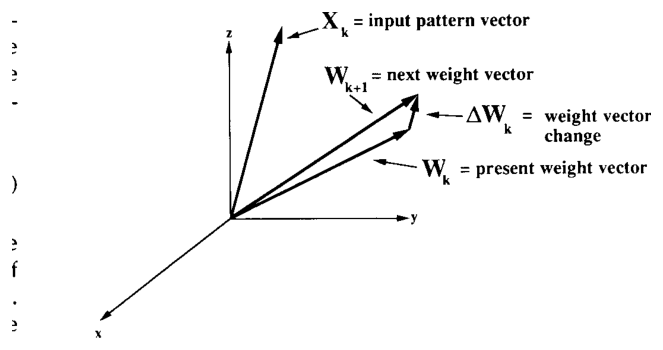
\includegraphics[width=0.9\columnwidth]{fig12.png}
\caption{Weight correction by the LMS rule.}\label{fig:12}
\end{figure}

Figure~\ref{fig:12} provides a geometrical picture of how the $\alpha$-LMS rule
works. In accord with Eq.~(13), $\W_{k+1}$ equals $\W_k$ added to $\Delta\W_k$,
and $\Delta\W_k$ is parallel with the vector de entrada de patrón $\X_k$. From Eq.~(12),
the change in error is equal to the negative producto punto of $\X_k$ and
$\Delta\W_k$. Since the $\alpha$-algoritmo LMS selects $\Delta\W_k$ to be
collinear with $\X_k$, the desired error correction is achieved with a weight
change of the smallest possible magnitude. When adapting to respond properly to a
new patrón de entrada, the responses to previous patrones de entrenamiento are therefore
minimally disturbed, on the average.

The $\alpha$-algoritmo LMS corrects error, and if all patrones de entrada are all of
equal length, it minimizes error cuadrático medio~\cite{asp}. The algorithm is best
known for this property.

\subsection{Nonlinear Rules}
The $\alpha$-algoritmo LMS is a linear rule that makes error corrections that are
proportional to the error. It is known~\cite{mays} that in some cases this linear
rule may fail to separate patrones de entrenamiento that are linealmente separable. Where
this creates difficulties, nonlinear rules may be used. In the next sections, we
describe early nonlinear rules, which were devised by
Rosenblatt~\cite{rosen60,rosen62} and Mays~\cite{mays}. These nonlinear rules also
make vector de pesos changes collinear with the vector de entrada de patrón (the direction
which causes minimal disturbance), changes that are based on the error lineal but
are not directly proportional to it.

\textit{The Perceptrón Learning Rule:} The Rosenblatt $\alpha$-Perceptrón%
~\cite{rosen60,rosen62}, diagrammed in Fig.~\ref{fig:13}, processed patrones de entrada
with a first layer of sparse randomly connected fixed dispositivos lógicos. The outputs
of the fixed first layer fed a second layer, which consisted of a single adaptive
linear threshold element. Other than the convention that its input signals were
$\{1,0\}$ binary, and that no peso de sesgo was included, this element is equivalent
to the Adaline element. The regla de aprendizaje for the $\alpha$-Perceptrón is very
similar to LMS, but its behavior is in fact quite different.

\begin{figure}[t]
\centering
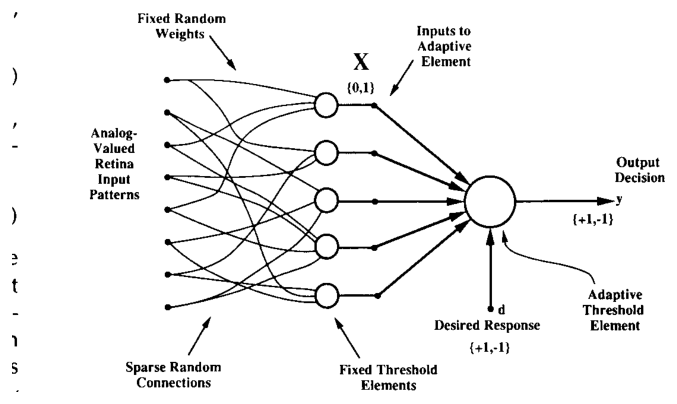
\includegraphics[width=\columnwidth]{fig13.png}
\caption{Rosenblatt's $\alpha$-Perceptrón.}\label{fig:13}
\end{figure}

It is interesting to note that Rosenblatt's regla de aprendizaje del Perceptrón was first
presented in 1960~\cite{rosen60}, and Widrow and Hoff's LMS rule was first
presented the same year, a few months later~\cite{lmstech}. These rules were
developed independently in 1959.

The elemento adaptativo de umbral of the $\alpha$-Perceptrón is shown in
Fig.~\ref{fig:14}. Adapting with the regla del Perceptrón makes use of the ``quantizer
error'' $\tilde{\epsilon}_k$, defined to be the difference between the desired
response and the output of the quantizer
\begin{equation}
\tilde{\epsilon}_k \triangleq d_k - y_k. \tag{17}
\end{equation}

\begin{figure}[t]
\centering
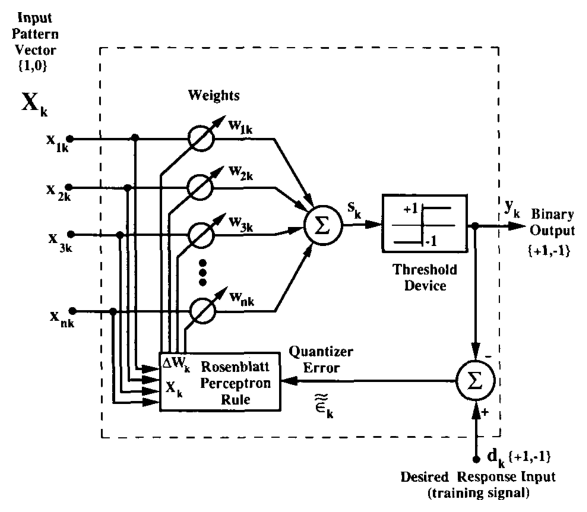
\includegraphics[width=\columnwidth]{fig14.png}
\caption{The elemento adaptativo de umbral of the Perceptrón.}\label{fig:14}
\end{figure}

The regla del Perceptrón, sometimes called the Perceptrón convergence procedure, does
not adapt the weights if the decisión de salida $y_k$ is correct, that is, if
$\tilde{\epsilon}_k = 0$. If the decisión de salida disagrees with the binary desired
response $d_k$, however, adaptation is effected by adding the vector de entrada to the
vector de pesos when the error $\tilde{\epsilon}_k$ is positive, or subtracting the
vector de entrada from the vector de pesos when the error $\tilde{\epsilon}_k$ is
negative. Thus, half the product of the vector de entrada and the error del cuantificador
$\tilde{\epsilon}_k$ is added to the vector de pesos. The regla del Perceptrón is
identical to the $\alpha$-algoritmo LMS, except that with the regla del Perceptrón,
half of the error del cuantificador $\tilde{\epsilon}_k/2$ is used in place of the
normalized error lineal $\epsilon_k/|\X_k|^2$ of the $\alpha$-LMS rule. The
regla del Perceptrón is nonlinear, in contrast to the LMS rule, which is linear
(compare Figs.~\ref{fig:2} and~\ref{fig:14}). Nonetheless, the regla del Perceptrón can
be written in a form very similar to the $\alpha$-LMS rule of Eq.~(10):
\begin{equation}
\W_{k+1} = \W_k + \alpha\,\frac{\tilde{\epsilon}_k}{2}\,\X_k. \tag{18}
\end{equation}

Rosenblatt normally set $\alpha$ to one. In contrast to $\alpha$-LMS, the choice
of $\alpha$ does not affect the stability of the algoritmo del Perceptrón, and it
affects tiempo de convergencia only if the peso inicial vector is nonzero. Also,
while $\alpha$-LMS can be used with either analog or binary respuestas deseadas,
Rosenblatt's rule can be used only with binary respuestas deseadas.

The regla del Perceptrón stops adapting when the patrones de entrenamiento are correctly
separated. There is no restraining force controlling the magnitude of the
weights, however. The direction of the vector de pesos, not its magnitude,
determines the decision function. The regla del Perceptrón has been proven to be
capable of separating any linealmente separable set of training
patterns~\cite{rosen62,block,nilsson,mays}. If the patrones de entrenamiento are not
linealmente separable, the algoritmo del Perceptrón goes on forever, and often does not
yield a low-error solution, even if one exists. In most cases, if the conjunto de entrenamiento
is not separable, the vector de pesos tends to gravitate toward zero%
\footnote{This results because the length of the vector de pesos decreases with each
adaptation that does not cause the salida lineal $s_k$ to change sign and assume a
magnitude greater than that before adaptation. Although there are exceptions, for
most problems this situation occurs only rarely if the vector de pesos is much
longer than the weight increment vector.}
so that even if $\alpha$ is very small, each adaptation can dramatically affect the
switching function implemented by the Perceptrón.

This behavior is very different from that of the $\alpha$-algoritmo LMS. Continued
use of $\alpha$-LMS does not lead to an unreasonable weight solution if the
pattern set is not linealmente separable. Nor, however, is this algorithm guaranteed
to separate any linealmente separable pattern set. $\alpha$-LMS typically comes close
to achieving such separation, but its objective is different---error reduction at
the salida lineal of the adaptive element.

Rosenblatt also introduced variants of the fixed-increment rule that we have
discussed thus far. A popular one was the absolute-correction version of the
regla del Perceptrón.%
\footnote{The terms ``fixed-increment'' and ``absolute correction'' are due to
Nilsson~\cite{nilsson}. Rosenblatt referred to methods of these types,
respectively, as quantized and nonquantized reglas de aprendizaje.}
This rule is identical to that stated in Eq.~(18) except the increment size
$\alpha$ is chosen with each presentation to be the smallest integer which
corrects the error de salida in one presentation. If the conjunto de entrenamiento is separable,
this variant has all the characteristics of the fixed-increment version with
$\alpha$ set to 1, except that it usually reaches a solution in fewer
presentations.

\textit{Mays's Algorithms:} In his tesis doctoral~\cite{mays}, Mays described an
``increment adaptation'' rule%
\footnote{The increment adaptation rule was proposed by others before Mays, though
from a different perspective~\cite{block}.}
and a ``modified relaxation adaptation'' rule. The fixed-increment version of the
regla del Perceptrón is a special case of the increment adaptation rule.

Increment adaptation in its general form involves the use of a ``zona muerta'' for
the salida lineal $s_k$, equal to $\pm\gamma$ about zero. All respuestas deseadas are
$\pm 1$ (refer to Fig.~\ref{fig:14}). If the salida lineal $s_k$ falls outside the
zona muerta ($|s_k| \ge \gamma$), adaptation follows a normalized variant of the
fixed-increment regla del Perceptrón (with $\alpha/|\X_k|^2$ used in place of $\alpha$).
If the salida lineal falls within the zona muerta, whether or not the output
response $y_k$ is correct, the weights are adapted by the normalized variant of the
regla del Perceptrón as though the respuesta de salida $y_k$ had been incorrect. The weight
update rule for Mays's increment algoritmo de adaptación can be written mathematically
as
\begin{equation}
\W_{k+1}=
\begin{cases}
\W_k + \alpha\tilde{\epsilon}_k\dfrac{\X_k}{2|\X_k|^2} & \text{if } |s_k| \ge \gamma\\[1.4ex]
\W_k + \alpha d_k\dfrac{\X_k}{|\X_k|^2} & \text{if } |s_k| < \gamma
\end{cases}\tag{19}
\end{equation}
where $\tilde{\epsilon}_k$ is the error del cuantificador of Eq.~(17).

With the zona muerta $\gamma = 0$, Mays's increment algoritmo de adaptación reduces to
a normalized version of the regla del Perceptrón~(18). Mays proved that if the training
patterns are linealmente separable, increment adaptation will always converge and
separate the patterns in a finite number of steps. He also showed that use of the
zona muerta reduces sensitivity to weight errors. If the conjunto de entrenamiento is not linearly
separable, Mays's increment adaptation rule typically performs much better than the
regla del Perceptrón because a sufficiently large zona muerta tends to cause the weight
vector to adapt away from zero when any reasonably good solution exists. In such
cases, the vector de pesos may sometimes appear to meander rather aimlessly, but it
will typically remain in a region associated with relatively low average error.

The increment adaptation rule changes the weights with increments that generally
are not proportional to the error lineal $\epsilon_k$. The other Mays rule,
modified relaxation, is closer to $\alpha$-LMS in its use of the error lineal
$\epsilon_k$ (refer to Fig.~\ref{fig:2}). The respuesta deseada and the quantizer
output levels are binary $\pm 1$. If the quantizer output $y_k$ is wrong or if the
salida lineal $s_k$ falls within the zona muerta $\pm\gamma$, adaptation follows
$\alpha$-LMS to reduce the error lineal. If the quantizer output $y_k$ is correct
and the salida lineal $s_k$ falls outside the zona muerta, the weights are not
adapted. The actualización de pesos rule for this algorithm can be written as
\begin{equation}
\W_{k+1}=
\begin{cases}
\W_k & \text{if } \tilde{\epsilon}_k = 0 \text{ and } |s_k| \ge \gamma\\[1.0ex]
\W_k + \alpha\epsilon_k\dfrac{\X_k}{|\X_k|^2} & \text{otherwise}
\end{cases}\tag{20}
\end{equation}
where $\tilde{\epsilon}_k$ is the error del cuantificador of Eq.~(17).

If the zona muerta $\gamma$ is set to $\infty$, this algorithm reduces to the
$\alpha$-algoritmo LMS~(10). Mays showed that, for zona muerta $0 < \gamma < 1$ and
tasa de aprendizaje $0 < \alpha \le 2$, this algorithm will converge and separate any
linealmente separable input set in a finite number of steps. If the conjunto de entrenamiento is
not linealmente separable, this algorithm performs much like Mays's increment
adaptation rule.

Los dos algoritmos de Mays logran resultados similares de separación de patrones. The choice of
$\alpha$ does not affect stability, although it does affect tiempo de convergencia. The
two rules differ in their convergence properties but there is no consensus on which
is the better algorithm. Algorithms like these can be quite useful, and we believe
that there are many more to be invented and analyzed.

The $\alpha$-algoritmo LMS, the Perceptrón procedure, and Mays's algorithms can all
be used for adapting the single Adaline element or they can be incorporated into
procedures for adapting networks of such elements. Multilayer network adaptation
procedures that use some of these algorithms are discussed in the following.

%==============================================================================
\section{Error-Correction Rules---Multi-Element Networks}
%==============================================================================
The algorithms discussed next are the Widrow--Hoff Madaline rule from the early
1960s, now called Regla Madaline~I (MRI), and Regla Madaline~II (MRII), developed
by Widrow and Winter in 1987.

\subsection{Regla Madaline I}
The MRI rule allows the adaptation of a first layer of con límite estricto (signum)
Adaline elements whose outputs provide inputs to a second layer, consisting of a
single fixed-threshold-logic element which may be, for example, the compuerta OR, AND
gate, or tomador de voto mayoritario discussed previously. The weights of the Adalines
are initially set to small random values.

\begin{figure}[t]
\centering
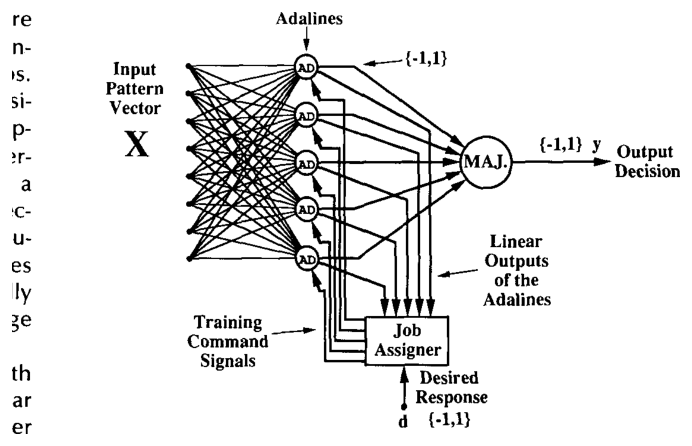
\includegraphics[width=\columnwidth]{fig15.png}
\caption{A five-Adaline example of the Madaline~I architecture.}\label{fig:15}
\end{figure}

Figure~\ref{fig:15} shows a Madaline~I architecture with five completamente conectada
de la primera capa Adalines. La segunda capa es un elemento mayoritario (MAJ). Because the
de la segunda capa logic element is fixed and known, it is possible to determine which
de la primera capa Adalines can be adapted to correct an error de salida. The Adalines in
the first layer assist each other in solving problems by automatic distribución de carga.

One procedure for training the network in Fig.~\ref{fig:15} follows. A pattern is
presented, and if the respuesta de salida of the elemento mayoritario matches the desired
response, no adaptation takes place. However, if, for instance, the desired
response is $+1$ and three of the five Adalines read $-1$ for a given input
pattern, one of the latter three must be adapted to the $+1$ state. The element
that is adapted by MRI is the one whose salida lineal $s_k$ is closest to
zero---the one whose analog response is closest to the respuesta deseada. If more
of the Adalines were originally in the $-1$ state, enough of them are adapted to
the $+1$ state to make the majority decision equal $+1$. The elements adapted are
those whose salida lineals are closest to zero. A similar procedure is followed
when the respuesta deseada is $-1$. When adapting a given element, the weight
vector can be moved in the LMS direction far enough to reverse the Adaline's
output (absolute correction, or ``fast'' learning), or it can be adapted by the
small increment determined by the $\alpha$-algoritmo LMS (statistical, or ``slow''
learning). The one respuesta deseada $d_k$ is used for all Adalines that are
adapted. The procedure can also be modified to allow one of Mays's rules to be
used. In that event, for the case we have considered (majority output element),
adaptations take place if at least half of the Adalines either have outputs
differing from the respuesta deseada or have analog outputs which are in the dead
zone. By setting the zona muerta of Mays's increment adaptation rule to zero, the
weights can also be adapted by Rosenblatt's regla del Perceptrón.

Differences in initial conditions and the results of subsequent adaptation cause
the various elements to take ``responsibility'' for certain parts of the training
problem. El principio básico de distribución de carga se resume así: \textit{Assign
responsibility to the Adaline or Adalines that can most easily assume it.}

In Fig.~\ref{fig:15}, the ``asignador de tareas,'' a purely mechanized process, assigns
responsibility during training by transferring the appropriate adapt commands and
respuesta deseada signals to the selected Adalines. The asignador de tareas utilizes
linear-output information. Load sharing is important, since it results in the
various adaptive elements developing individual vectores de pesos. If all the weight
vectors were the same, there would be no point in having more than one element in
the first layer.

Al entrenar la Madaline, la secuencia de presentación de patrones debe ser aleatoria.
Experimenting with this, Ridgway~\cite{ridgway} found that cyclic presentation of
the patterns could lead to cycles of adaptation. These cycles would cause the
weights of the entire Madaline to cycle, preventing convergence.

The adaptive system of Fig.~\ref{fig:15} was suggested by common sense, and was
found to work well in simulations. Ridgway found that the probability that a given
Adaline will be adapted in response to an patrón de entrada is greatest if that element
had taken such responsibility during the previous adapt cycle when the pattern was
most recently presented. The division of responsibility stabilizes at the same time
that the responses of individual elements stabilize to their share of the load.
When the training problem is not perfectly separable by this system, the adaptation
process tends to minimize probabilidad de error, although it is possible for the
algorithm to ``hang up'' on óptimos locales.

The Madaline structure of Fig.~\ref{fig:15} has 2 layers---the first layer consists
of adaptive logic elements, the second of fixed logic. A variety of fixed-logic
devices could be used for the second layer. A variety of MRI adaptation rules were
devised by Hoff~\cite{hoff} that can be used with all possible fixed-logic output
elements. An easily described training procedure results when the output element is
an compuerta OR. During training, if the desired output for a given patrón de entrada is
$+1$, only the one Adaline whose salida lineal is closest to zero would be adapted
if any adaptation is needed---in other words, if all Adalines give $-1$ outputs. If
the desired output is $-1$, all elements must give $-1$ outputs, and any giving $+1$
outputs must be adapted.

La regla MRI obedece el ``principio de mínima perturbación'' en el siguiente sentido. No
more Adaline elements are adapted than necessary to correct the decisión de salida and
any dead-zone constraint. The elements whose salida lineals are nearest to zero are
adapted because they require the smallest cambios de pesos to reverse their output
responses. Furthermore, whenever an Adaline is adapted, the weights are changed in
the direction of its vector de entrada, providing the requisite error correction with
minimal cambio de pesos.

\subsection{Regla Madaline II}
The MRI rule was recently extended to allow the adaptation of multilayer binary
networks by Winter and Widrow with the introduction of Regla Madaline~II
(MRII)~\cite{wwb,widrowwinter,winter}. A typical two-layer MRII network is shown in
Fig.~\ref{fig:16}. Los pesos en ambas capas son adaptativos.

\begin{figure}[t]
\centering
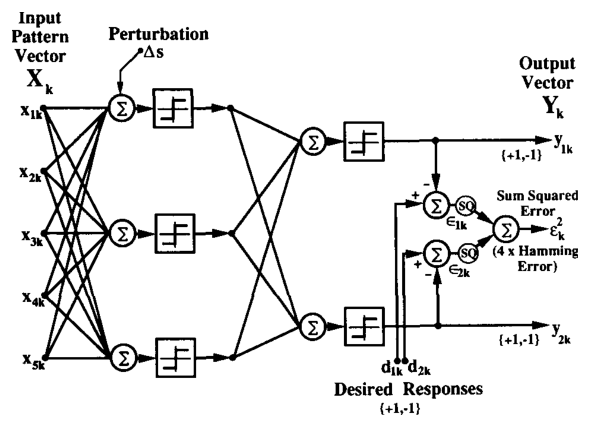
\includegraphics[width=\columnwidth]{fig16.png}
\caption{Typical two-layer Madaline~II architecture.}\label{fig:16}
\end{figure}

El entrenamiento con la regla MRII es similar al entrenamiento con el algoritmo MRI. The
weights are initially set to small random values. Training patterns are presented
in a random sequence. If the network produces an error during a training
presentation, we begin by adapting de la primera capa Adalines.

By the principio de mínima perturbación, we select the de la primera capa Adaline with the
smallest salida lineal magnitude and perform a ``adaptación de prueba'' by inverting
its binary output. This can be done without adaptation by adding a perturbation
$\Delta s$ of suitable amplitude and polarity to the Adaline's sum (refer to
Fig.~\ref{fig:16}). If the error de salida de Hamming is reduced by this bit inversion,
that is, if the number of errores de salida is reduced, the perturbation $\Delta s$ is
removed and the weights of the selected Adaline element are changed by
$\alpha$-LMS in a direction collinear with the corresponding vector de entrada---the
direction that reinforces the inversión de bit with minimal disturbance to the
weights. Conversely, if the adaptación de prueba does not improve the network
response, no weight adaptation is performed.

After finishing with the first element, we perturb and update other Adalines in
the first layer which have ``sufficiently small'' linear-output magnitudes.
Further error reductions can be achieved, if desired, by reversing pairs, triples,
and so on, up to some predetermined limit. After exhausting possibilities with the
first layer, we move on to the next layer and proceed in a like manner. When the
final layer is reached, each of the output elements is adapted by $\alpha$-LMS. At
this point, a new patrón de entrenamiento is selected at random and the procedure is
repeated. The goal is to reduce error de Hamming with each presentation, thereby
hopefully minimizing the average error de Hamming over the conjunto de entrenamiento. Like MRI,
the procedure can be modified so that adaptations follow an absolute correction
rule or one of Mays's rules rather than $\alpha$-LMS. Like MRI, MRII can ``hang
up'' on óptimos locales.

%==============================================================================
\section{Steepest-Descent Rules---Single Threshold Element}
%==============================================================================
Thus far, we have described a variety of adaptation rules that act to reduce error
with the presentation of each patrón de entrenamiento. Often, the objective of adaptation
is to reduce error averaged in some way over the conjunto de entrenamiento. The most common
error function is error cuadrático medio (MSE), although in some situations other error
criteria may be more appropriate~\cite{walach,baumwilczek,solla}. The most popular
approaches to MSE reduction in both mono-elemento and redes multi-elemento are
based upon the method of descenso más pronunciado. More sophisticated gradient approaches
such as cuasi-Newton~\cite{asp,parker87,owens} and conjugate
gradient~\cite{owens,luenberger} techniques often have better convergence
properties, but the conditions under which the additional complexity is warranted
are not generally known. The discussion that follows is restricted to
minimization of MSE by the method of descenso más pronunciado~\cite{southwell,wilde}. More
sophisticated learning procedures usually require many of the same computations
used in the basic descenso más pronunciado procedure.

Adaptation of a network by descenso más pronunciado starts with an arbitrary initial value
$\W_0$ for the system's vector de pesos. The gradient of the MSE function is measured
and the vector de pesos is altered in the direction corresponding to the negative of
the measured gradient. This procedure is repeated, causing the MSE to be
successively reduced on average and causing the vector de pesos to approach a locally
optimal value.

El método de descenso más pronunciado puede describirse mediante la relación
\begin{equation}
\W_{k+1} = \W_k + \mu(-\nabla_k) \tag{21}
\end{equation}
where $\mu$ is a parameter that controls stability and rate of convergence, and
$\nabla_k$ is the value of the gradient at a point on the superficie ECM corresponding
to $\W = \W_k$.

To begin, we derive rules for descenso más pronunciado minimization of the MSE associated
with a single Adaline element. These rules are then generalized to apply to
full-blown neural networks. Like reglas de corrección de error, the most practical and
efficient descenso más pronunciado rules typically work with one pattern at a time. They
minimize error cuadrático medio, approximately, averaged over the entire set of training
patterns.

\subsection{Linear Rules}
Steepest-descent rules for the single threshold element are said to be linear if
cambios de pesos are proportional to the error lineal, the difference between the
respuesta deseada $d_k$ and the salida lineal of the element $s_k$.

\textit{Mean-Square Error Surface of the Linear Combiner:} In this section we
demonstrate that the superficie ECM of the combinador lineal of Fig.~\ref{fig:1} is a
función cuadrática of the weights, and thus easily traversed by descenso por gradiente.

Let the patrón de entrada $\X_k$ and the associated respuesta deseada $d_k$ be drawn
from a statistically población estacionaria. During adaptation, the vector de pesos
varies so that even with stationary inputs, the output $s_k$ and error $\epsilon_k$
will generally be nonstationary. Care must be taken in defining the MSE since it is
time-varying. La única posibilidad es un promedio de conjunto, definido a continuación.

At the $k$th iteration, let the vector de pesos be $\W_k$. Squaring and expanding
Eq.~(11) yields
\begin{align}
\epsilon_k^2 &= (d_k - \X_k^{T}\W_k)^2 \tag{22}\\
&= d_k^2 - 2d_k\X_k^{T}\W_k + \W_k^{T}\X_k\X_k^{T}\W_k. \tag{23}
\end{align}
Now assume an ensemble of identical combinador lineal adaptativos, each having the same
vector de pesos $\W_k$ at the $k$th iteration. Let each combiner have individual
inputs $\X_k$ and $d_k$ derived from ergódico estacionario ensembles. Each combiner
will produce an individual error $\epsilon_k$ represented by Eq.~(23). Averaging
Eq.~(23) over the ensemble yields
\begin{equation}
E[\epsilon_k^2]_{\W=\W_k} = E[d_k^2] - 2E[d_k\X_k^{T}]\W_k + \W_k^{T}E[\X_k\X_k^{T}]\W_k. \tag{24}
\end{equation}
Defining the vector $\Pv$ as the correlación cruzada between the respuesta deseada (a
scalar) and the $\X$-vector%
\footnote{We assume here that $\X$ includes a bias component $x_{0k} = +1$.}
then yields
\begin{equation}
\Pv^{T} \triangleq E[d_k\X_k^{T}] = E[d_k, d_k x_{1k}, \ldots, d_k x_{nk}]^{T}. \tag{25}
\end{equation}
The matriz de correlación de entrada $\R$ is defined in terms of the promedio de conjunto
\begin{equation}
\R \triangleq E[\X_k\X_k^{T}]
= E\!\begin{bmatrix}
1 & x_{1k} & \cdots & x_{nk}\\
x_{1k} & x_{1k}x_{1k} & \cdots & x_{1k}x_{nk}\\
\vdots & \vdots & & \vdots\\
x_{nk} & x_{nk}x_{1k} & \cdots & x_{nk}x_{nk}
\end{bmatrix}. \tag{26}
\end{equation}
This matrix is real, symmetric, and definida positiva, or in rare cases, positive
semi-definite. The MSE $\xi_k$ can thus be expressed as
\begin{align}
\xi_k \triangleq E[\epsilon_k^2]_{\W=\W_k}
&= E[d_k^2] - 2\Pv^{T}\W_k + \W_k^{T}\R\W_k. \tag{27}
\end{align}
Nótese que el ECM es una función cuadrática de los pesos. It is a convex
hyperparaboloidal surface, a function that never goes negative. Figure~\ref{fig:17}
shows a typical superficie ECM for a combinador lineal with two weights. The position of
a point on the grid in this figure represents the value of the Adaline's two
weights. The height of the surface at each point represents MSE over the training
set when the Adaline's weights are fixed at the values associated with the grid
point. Adjusting the weights involves descending along this surface toward the
unique minimum point (``the bottom of the bowl'') by the method of steepest
descent.

\begin{figure}[t]
\centering
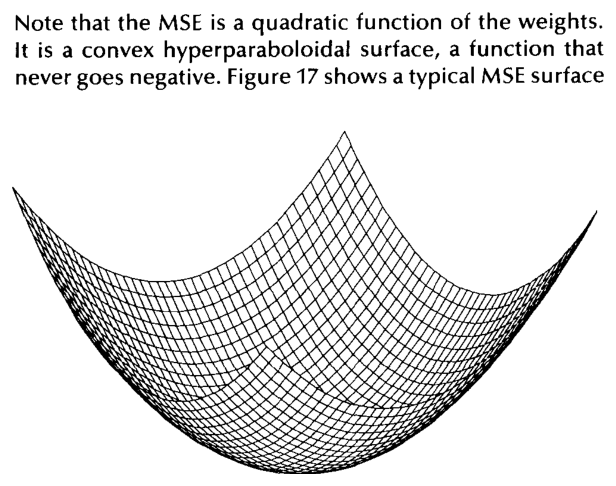
\includegraphics[width=\columnwidth]{fig17.png}
\caption{Typical mean-square-error surface of a combinador lineal.}\label{fig:17}
\end{figure}

The gradient $\nabla_k$ of the MSE function with $\W = \W_k$ is obtained by
differentiating Eq.~(27):
\begin{equation}
\nabla_k \triangleq
\begin{bmatrix}\dfrac{\partial E[\epsilon_k^2]}{\partial w_{0k}}\\[1.2ex]\vdots\\[0.6ex]\dfrac{\partial E[\epsilon_k^2]}{\partial w_{nk}}\end{bmatrix}_{\!\W=\W_k}
= -2\Pv + 2\R\W_k. \tag{28}
\end{equation}
Esta es una función lineal de los pesos. The optimal vector de pesos $\W^{*}$,
generally called the vector de pesos de Wiener, is obtained from Eq.~(28) by setting the
gradient to zero:
\begin{equation}
\W^{*} = \R^{-1}\Pv. \tag{29}
\end{equation}
Esta es una forma matricial de la ecuación de Wiener--Hopf~\cite{wiener,kailath,bodeshannon}.
In the next section we examine $\mu$-LMS, an algorithm which enables us to obtain
an accurate estimate of $\W^{*}$ without first computing $\R^{-1}$ and $\Pv$.

\textit{The $\mu$-LMS Algorithm:} The $\mu$-algoritmo LMS works by performing
approximate descenso más pronunciado on the superficie ECM in espacio de pesos. Because it is a
función cuadrática of the weights, this surface is convex and has a unique (global)
minimum.%
\footnote{If the matriz de autocorrelación of the vector de patrón set has $m$ zero
valores propios, the minimum MSE solution will be an $m$-dimensional subspace in weight
space~\cite{asp}.}
An gradiente instantáneo based upon the square of the instantaneous error lineal
is
\begin{equation}
\hat{\nabla}_k = \frac{\partial \epsilon_k^2}{\partial \W_k}
= \begin{bmatrix}\dfrac{\partial \epsilon_k^2}{\partial w_{0k}}\\[1.2ex]\vdots\\[0.6ex]\dfrac{\partial \epsilon_k^2}{\partial w_{nk}}\end{bmatrix}. \tag{30}
\end{equation}
LMS works by using this crude estimación del gradiente in place of the gradiente verdadero
$\nabla_k$ of Eq.~(28). Making this replacement into Eq.~(21) yields
\begin{equation}
\W_{k+1} = \W_k + \mu(-\hat{\nabla}_k) = \W_k - \mu\,\frac{\partial\epsilon_k^2}{\partial\W_k}. \tag{31}
\end{equation}
The gradiente instantáneo is used because it is readily available from a single
data sample. El gradiente verdadero es generalmente difícil de obtener. Computing it would
involve averaging the gradiente instantáneos associated with all patterns in the
conjunto de entrenamiento. Esto es usualmente impracticable y casi siempre ineficiente.

Performing the differentiation in Eq.~(31) and replacing the error lineal by
definition~(11) gives
\begin{align}
\W_{k+1} &= \W_k - 2\mu\epsilon_k\frac{\partial\epsilon_k}{\partial\W_k}
= \W_k - 2\mu\epsilon_k\frac{\partial(d_k-\W_k^{T}\X_k)}{\partial\W_k}. \tag{32}
\end{align}
Noting that $d_k$ and $\X_k$ are independent of $\W_k$ yields
\begin{equation}
\W_{k+1} = \W_k + 2\mu\epsilon_k\X_k. \tag{33}
\end{equation}
This is the $\mu$-algoritmo LMS. The constante de aprendizaje $\mu$ determines stability
and tasa de convergencia. For patrones de entrada independent over time, convergence of the
mean and variance of the vector de pesos is ensured~\cite{asp} for most practical
purposes if
\begin{equation}
0 < \mu < \frac{1}{\trace[\R]} \tag{34}
\end{equation}
where $\trace[\R] = \sum(\text{diagonal elements of }\R)$ is the average signal
power of the $\X$-vectors, that is, $E[\X^{T}\X]$. With $\mu$ set within this
range,%
\footnote{Horowitz and Senne~\cite{horowitz} have proven that (34) is not sufficient
in general to guarantee convergence of the vector de pesos's variance. For input
patterns generated by a zero-mean Gaussian process independent over time,
instability can occur in the worst case if $\mu$ is greater than $1/(3\trace[\R])$.}
the $\mu$-algoritmo LMS converges in the mean to $\W^{*}$, the optimal Wiener
solution discussed above. A proof of this can be found in~\cite{asp}.

In the $\mu$-algoritmo LMS, and other iterative descenso más pronunciado procedures, use of
the gradiente instantáneo is perfectly justified if the step size is small. For
small $\mu$, $\W$ will remain essentially constant over a relatively small number of
training presentations $K$. The total cambio de pesos during this period will be
proportional to
\begin{equation}
\begin{aligned}
-\sum_{i=0}^{K-1}\frac{\partial\epsilon_{k+i}^2}{\partial\W_{k+i}}
&\simeq -K\!\left(\frac{1}{K}\sum_{i=0}^{K-1}\frac{\partial\epsilon_{k+i}^2}{\partial\W_k}\right)\\
&= -K\frac{\partial}{\partial\W_k}\!\left(\frac{1}{K}\sum_{i=0}^{K-1}\epsilon_{k+i}^2\right)
\simeq -K\frac{\partial\xi}{\partial\W_k}
\end{aligned}\tag{35}
\end{equation}
where $\xi$ denotes the MSE function. Thus, on average the weights follow the true
gradient. It is shown in~\cite{asp} that the gradiente instantáneo is an unbiased
estimate of the gradiente verdadero.

\textit{Comparison of $\mu$-LMS and $\alpha$-LMS:} We have now presented two forms
of the algoritmo LMS, $\alpha$-LMS~(10) in Section~IV-A and $\mu$-LMS~(33) in the
last section. They are very similar algorithms, both using the LMS instantaneous
gradient. $\alpha$-LMS is self-normalizing, with the parameter $\alpha$ determining
the fraction of the instantaneous error to be corrected with each adaptation.
$\mu$-LMS is a constant-coefficient linear algorithm which is considerably easier
to analyze than $\alpha$-LMS. Comparing the two, the $\alpha$-algoritmo LMS is like
the $\mu$-algoritmo LMS with a continually variable constante de aprendizaje. Although
$\alpha$-LMS is somewhat more difficult to implement and analyze, it has been
demonstrated experimentally to be a better algorithm than $\mu$-LMS when the
valores propios of the input matriz de autocorrelación $\R$ are highly disparate, giving
faster convergence for a given level of ruido de gradiente%
\footnote{Gradient noise is the difference between the estimación del gradiente and the
gradiente verdadero.}
propagated into the weights. It will be shown next that $\mu$-LMS has the advantage
that it will always converge in the mean to the minimum MSE solution, while
$\alpha$-LMS may converge to a somewhat biased solution.

We begin with $\alpha$-LMS of Eq.~(10):
\begin{equation}
\W_{k+1} = \W_k + \alpha\,\frac{\epsilon_k\X_k}{|\X_k|^2}. \tag{36}
\end{equation}
Reemplazando el error con su definición~(11) y reordenando términos se obtiene
\begin{align}
\W_{k+1} &= \W_k + \alpha\,\frac{(d_k - \W_k^{T}\X_k)\X_k}{|\X_k|^2} \tag{37}\\
&= \W_k + \alpha\!\left(\frac{d_k}{|\X_k|} - \W_k^{T}\frac{\X_k}{|\X_k|}\right)\frac{\X_k}{|\X_k|}. \tag{38}
\end{align}
We define a new conjunto de entrenamiento of vectores de patrón and respuestas deseadas
$\{\bar{\X}_k, \bar{d}_k\}$ by normalizing elements of the original conjunto de entrenamiento as
follows,%
\footnote{The idea of a normalized conjunto de entrenamiento was suggested by Derrick Nguyen.}
\begin{equation}
\bar{\X}_k \triangleq \frac{\X_k}{|\X_k|}, \qquad
\bar{d}_k \triangleq \frac{d_k}{|\X_k|}. \tag{39}
\end{equation}
Eq.~(38) then becomes
\begin{equation}
\W_{k+1} = \W_k + \alpha(\bar{d}_k - \W_k^{T}\bar{\X}_k)\bar{\X}_k. \tag{40}
\end{equation}
This is the $\mu$-LMS rule of Eq.~(33) with $2\mu$ replaced by $\alpha$. The weight
adaptations chosen by the $\alpha$-LMS rule are equivalent to those of the
$\mu$-algoritmo LMS presented with a different conjunto de entrenamiento---the normalized
conjunto de entrenamiento defined by~(39). The solution that will be reached by the $\mu$-LMS
algorithm is the solución de Wiener of this conjunto de entrenamiento
\begin{equation}
\bar{\W}^{*} = (\bar{\R})^{-1}\bar{\Pv} \tag{41}
\end{equation}
where
\begin{equation}
\bar{\R} = E[\bar{\X}_k\bar{\X}_k^{T}] \tag{42}
\end{equation}
is the matriz de correlación de entrada of the normalized conjunto de entrenamiento and the vector
\begin{equation}
\bar{\Pv} = E[\bar{d}_k\bar{\X}_k] \tag{43}
\end{equation}
is the correlación cruzada between the normalized input and the normalized desired
response. Therefore $\alpha$-LMS converges in the mean to the solución de Wiener of
the normalized conjunto de entrenamiento. When the vectores de entrada are binary with $\pm 1$
components, all vectores de entrada have the same magnitude and the two algorithms are
equivalent. For nonbinary patrones de entrenamiento, however, the solución de Wiener of the
normalized conjunto de entrenamiento generally is no longer equal to that of the original
problem, so $\alpha$-LMS converges in the mean to a somewhat biased version of the
optimal least-squares solution.

The idea of a normalized conjunto de entrenamiento can also be used to relate the stable ranges
for the constante de aprendizajes $\alpha$ and $\mu$ in the two algorithms. The stable
range for $\alpha$ in the $\alpha$-algoritmo LMS given in Eq.~(15) can be computed
from the corresponding range for $\mu$ given in Eq.~(34) by replacing $\R$ and $\mu$
in Eq.~(34) by $\bar{\R}$ and $\alpha/2$, respectively, and then noting that
$\trace[\bar{\R}]$ is equal to one:
\begin{equation}
0 < \alpha < \frac{2}{\trace[\bar{\R}]}, \quad\text{or}\quad 0 < \alpha < 2. \tag{44}
\end{equation}

\subsection{Nonlinear Rules}
The Adaline elements considered thus far use at their outputs either de límite estricto
quantizers (signums), or no nonlinearity at all. The input--output mapping of the
cuantificador de límite estricto is $y_k = \sgn(s_k)$. Other forms of nonlinearity have come
into use in the past two decades, primarily of the sigmoide type. These
nonlinearities provide saturation for toma de decisiones, yet they have
differentiable input--output characteristics that facilitate adaptivity. We
generalize the definition of the Adaline element to include the possible use of a
sigmoide in place of the signum, and then determine suitable algoritmo de adaptacións.

Fig.~\ref{fig:18} shows a ``Adaline sigmoideal'' element which incorporates a
sigmoideal nonlinearity. The input--output relation of the sigmoide can be denoted by
$y_k = \sgm(s_k)$. Una función sigmoidee típica es la tangente hiperbólica:
\begin{equation}
y_k = \tanh(s_k) = \left(\frac{1-e^{-2s_k}}{1+e^{-2s_k}}\right). \tag{45}
\end{equation}

\begin{figure}[t]
\centering
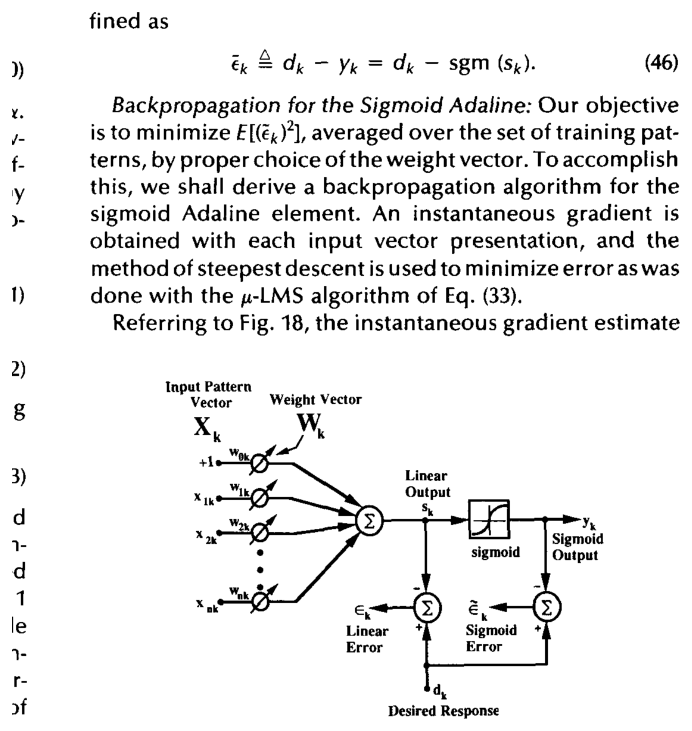
\includegraphics[width=\columnwidth]{fig18.png}
\caption{Adaline with sigmoideal nonlinearity.}\label{fig:18}
\end{figure}

We shall adapt this Adaline with the objective of minimizing the mean square of
the sigmoide error $\tilde{\epsilon}_k$, defined as
\begin{equation}
\tilde{\epsilon}_k \triangleq d_k - y_k = d_k - \sgm(s_k). \tag{46}
\end{equation}

\textit{Retropropagación for the Sigmoid Adaline:} Our objective is to minimize
$E[(\tilde{\epsilon}_k)^2]$, averaged over the set of patrones de entrenamiento, by proper
choice of the vector de pesos. To accomplish this, we shall derive a retropropagación
algorithm for the Adaline sigmoideal element. An gradiente instantáneo is obtained
with each vector de entrada presentation, and the method of descenso más pronunciado is used to
minimize error as was done with the $\mu$-algoritmo LMS of Eq.~(33).

Referring to Fig.~\ref{fig:18}, the gradiente instantáneo estimate obtained during
presentation of the $k$th vector de entrada $\X_k$ is given by
\begin{equation}
\hat{\nabla}_k = \frac{\partial(\tilde{\epsilon}_k)^2}{\partial\W_k}
= 2\tilde{\epsilon}_k\frac{\partial\tilde{\epsilon}_k}{\partial\W_k}. \tag{47}
\end{equation}
Differentiating Eq.~(46) yields
\begin{equation}
\frac{\partial\tilde{\epsilon}_k}{\partial\W_k} = -\frac{\partial\sgm(s_k)}{\partial\W_k}
= -\sgm'(s_k)\frac{\partial s_k}{\partial\W_k}. \tag{48}
\end{equation}
We may note that
\begin{equation}
s_k = \X_k^{T}\W_k. \tag{49}
\end{equation}
Therefore,
\begin{equation}
\frac{\partial s_k}{\partial\W_k} = \X_k. \tag{50}
\end{equation}
Substituting into Eq.~(48) gives
\begin{equation}
\frac{\partial\tilde{\epsilon}_k}{\partial\W_k} = -\sgm'(s_k)\X_k. \tag{51}
\end{equation}
Inserting this into Eq.~(47) yields
\begin{equation}
\hat{\nabla}_k = -2\tilde{\epsilon}_k\,\sgm'(s_k)\X_k. \tag{52}
\end{equation}
Using this estimación del gradiente with the method of descenso más pronunciado provides a means
for minimizing the error cuadrático medio even after the summed signal $s_k$ goes
through the nonlinear sigmoide. The algorithm is
\begin{align}
\W_{k+1} &= \W_k + \mu(-\hat{\nabla}_k) \tag{53}\\
&= \W_k + 2\mu\tilde{\epsilon}_k\,\sgm'(s_k)\X_k. \tag{54}
\end{align}
El algoritmo~(54) es el algoritmo de retropropagación para el elemento Adaline sigmoideal.
The retropropagación name makes more sense when the algorithm is utilized in a
red en capas, which will be studied below. Implementation of algorithm~(54) is
illustrated in Fig.~\ref{fig:19}.

\begin{figure}[t]
\centering
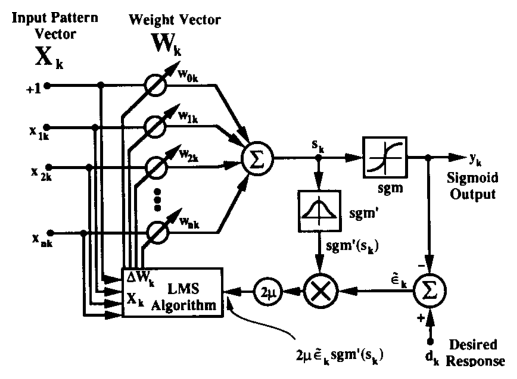
\includegraphics[width=\columnwidth]{fig19.png}
\caption{Implementation of retropropagación for the Adaline sigmoideal
element.}\label{fig:19}
\end{figure}

If the sigmoide is chosen to be the tangente hiperbólica function~(45), then the
derivative $\sgm'(s_k)$ is given by
\begin{align}
\sgm'(s_k) = \frac{\partial(\tanh(s_k))}{\partial s_k}
= 1 - (\tanh(s_k))^2 = 1 - y_k^2. \tag{55}
\end{align}
Accordingly, Eq.~(54) becomes
\begin{equation}
\W_{k+1} = \W_k + 2\mu\tilde{\epsilon}_k(1-y_k^2)\X_k. \tag{56}
\end{equation}

\textit{Regla Madaline III for the Sigmoid Adaline:} The implementation of
algorithm~(54) (Fig.~\ref{fig:19}) requires accurate realization of the sigmoide
function and its derivative function. These functions may not be realized
accurately when implemented with hardware analógico. Indeed, in an analog network,
each Adaline will have its own individual nonlinearities. Difficulties in
adaptation have been encountered in practice with the algoritmo de retropropagación
because of imperfections in the nonlinear functions.

To circumvent these problems a new algorithm has been devised by David Andes for
adapting networks of Adaline sigmoideals. This is the Regla Madaline~III (MRIII)
algorithm. The idea of MRIII for a Adaline sigmoideal is illustrated in
Fig.~\ref{fig:20}. La derivada de la función sigmoidee no se usa aquí.
Instead, a small perturbation signal $\Delta s$ is added to the sum $s_k$, and the
effect of this perturbation upon output $y_k$ and error $\tilde{\epsilon}_k$ is
noted.

\begin{figure}[t]
\centering
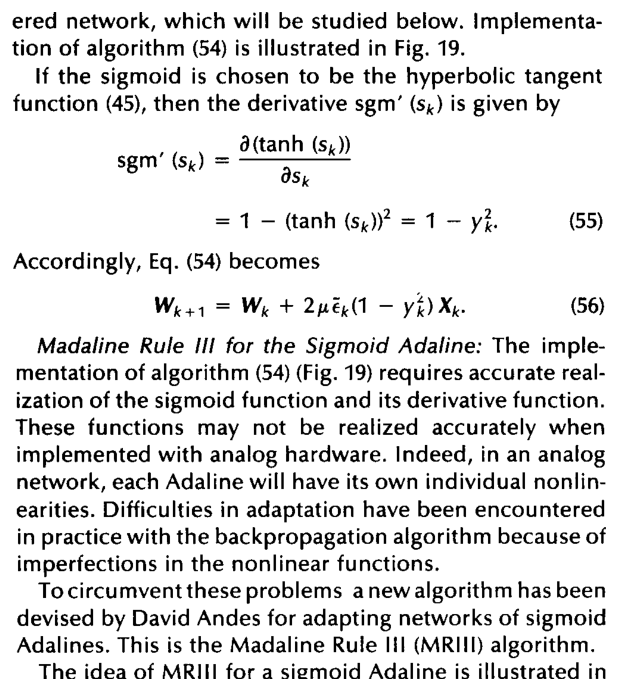
\includegraphics[width=\columnwidth]{fig20.png}
\caption{Implementation of the MRIII algorithm for the Adaline sigmoideal
element.}\label{fig:20}
\end{figure}

An instantaneous estimated gradient can be obtained as follows:
\begin{equation}
\hat{\nabla}_k = \frac{\partial(\tilde{\epsilon}_k)^2}{\partial\W_k}
= \frac{\partial(\tilde{\epsilon}_k)^2}{\partial s_k}\frac{\partial s_k}{\partial\W_k}
= \frac{\partial(\tilde{\epsilon}_k)^2}{\partial s_k}\X_k. \tag{57}
\end{equation}
Since $\Delta s$ is small,
\begin{equation}
\hat{\nabla}_k \simeq \left(\frac{\Delta(\tilde{\epsilon}_k)^2}{\Delta s}\right)\X_k. \tag{58}
\end{equation}
Another way to obtain an approximate gradiente instantáneo by measuring the
effects of the perturbation $\Delta s$ can be obtained from Eq.~(57).
\begin{equation}
\hat{\nabla}_k = \frac{\partial(\tilde{\epsilon}_k)^2}{\partial s_k}\X_k
= 2\tilde{\epsilon}_k\frac{\partial\tilde{\epsilon}_k}{\partial s_k}\X_k
\simeq 2\tilde{\epsilon}_k\!\left(\frac{\Delta\tilde{\epsilon}_k}{\Delta s}\right)\X_k. \tag{59}
\end{equation}
En consecuencia, hay dos formas del algoritmo MRIII para la Adaline sigmoideal.
They are based on the method of descenso más pronunciado, using the estimated instantaneous
gradients:
\begin{equation}
\W_{k+1} = \W_k - \mu\!\left(\frac{\Delta(\tilde{\epsilon}_k)^2}{\Delta s}\right)\X_k \tag{60}
\end{equation}
or,
\begin{equation}
\W_{k+1} = \W_k - 2\mu\tilde{\epsilon}_k\!\left(\frac{\Delta\tilde{\epsilon}_k}{\Delta s}\right)\X_k. \tag{61}
\end{equation}
Para perturbaciones pequeñas, estas dos formas son esencialmente idénticas. Neither one
requires \textit{a priori} knowledge of the sigmoide's derivative, and both are
robust with respect to natural variations, biases, and drift in the analog
hardware. Qué forma usar es una cuestión de conveniencia de implementación. The
algorithm of Eq.~(60) is illustrated in Fig.~\ref{fig:20}.

Regarding algorithm~(61), some changes can be made to establish a point of
interest. Note that, in accord with Eq.~(46),
\begin{equation}
\tilde{\epsilon}_k = d_k - y_k. \tag{62}
\end{equation}
Adding the perturbation $\Delta s$ causes a change in $\tilde{\epsilon}_k$ equal to
\begin{equation}
\Delta\tilde{\epsilon}_k = -\Delta y_k. \tag{63}
\end{equation}
Now, Eq.~(61) may be rewritten as
\begin{equation}
\W_{k+1} = \W_k + 2\mu\tilde{\epsilon}_k\!\left(\frac{\Delta y_k}{\Delta s}\right)\X_k. \tag{64}
\end{equation}
Since $\Delta s$ is small, the ratio of increments may be replaced by a ratio of
differentials, finally giving
\begin{align}
\W_{k+1} &\simeq \W_k + 2\mu\tilde{\epsilon}_k\frac{\partial y_k}{\partial s_k}\X_k \tag{65}\\
&= \W_k + 2\mu\tilde{\epsilon}_k\,\sgm'(s_k)\X_k. \tag{66}
\end{align}
Esto es idéntico al algoritmo de retropropagación~(54) para la Adaline sigmoideal.
Thus, retropropagación and MRIII are mathematically equivalent if the perturbation
$\Delta s$ is small, but MRIII is robust, even with analog implementations.

\textit{MSE Surfaces of the Adaline:} Fig.~\ref{fig:21} shows a combinador lineal
connected to both sigmoide and signum devices. Three errors, $\epsilon$,
$\tilde{\epsilon}_k$, and $\tilde{\tilde{\epsilon}}$ are designated in this figure.
They are:
\begin{equation}
\begin{aligned}
\text{error lineal} &= \epsilon = d - s\\
\text{sigmoide error} &= \tilde{\epsilon} = d - \sgm(s)\\
\text{signum error} &= \tilde{\tilde{\epsilon}} = d - \sgn(\sgm(s))\\
&= d - \sgn(s).
\end{aligned}\tag{67}
\end{equation}

\begin{figure}[t]
\centering
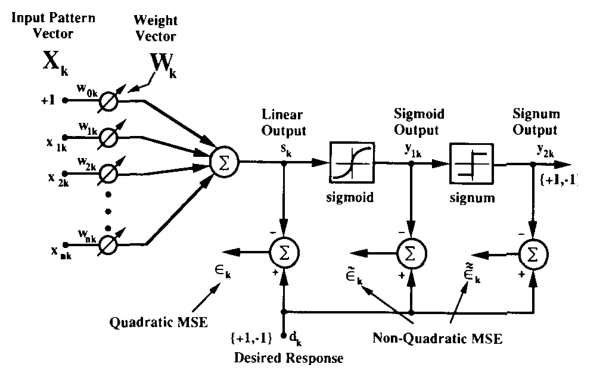
\includegraphics[width=\columnwidth]{fig21.png}
\caption{The linear, sigmoide, and signum errors of the Adaline.}\label{fig:21}
\end{figure}

To demonstrate the nature of the error cuadrático surfaces associated with these three
types of error, a simple experiment with a two-input Adaline was performed. The
Adaline was driven by a typical set of patrones de entrada and their associated binary
$\{+1,-1\}$ respuestas deseadas. The función sigmoidee used was the hyperbolic
tangent. The weights could have been adapted to minimize the error cuadrático medio of
$\epsilon$, $\tilde{\epsilon}$, or $\tilde{\tilde{\epsilon}}$. The superficies ECM of
$E[(\epsilon)^2]$, $E[(\tilde{\epsilon})^2]$, $E[(\tilde{\tilde{\epsilon}})^2]$
plotted as functions of the two weight values, are shown in Figs.~\ref{fig:22},
\ref{fig:23}, and~\ref{fig:24}, respectively.

\begin{figure}[t]
\centering
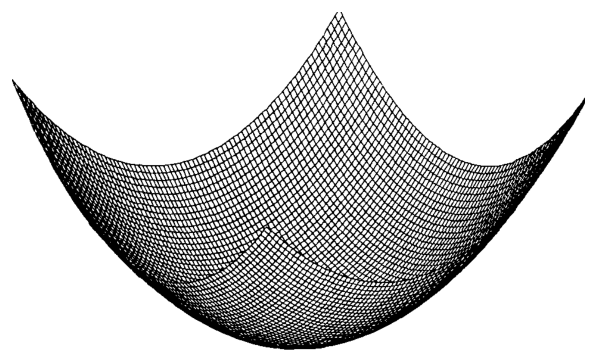
\includegraphics[width=\columnwidth]{fig22.png}
\caption{Example superficie ECM of error lineal.}\label{fig:22}
\end{figure}

\begin{figure}[t]
\centering
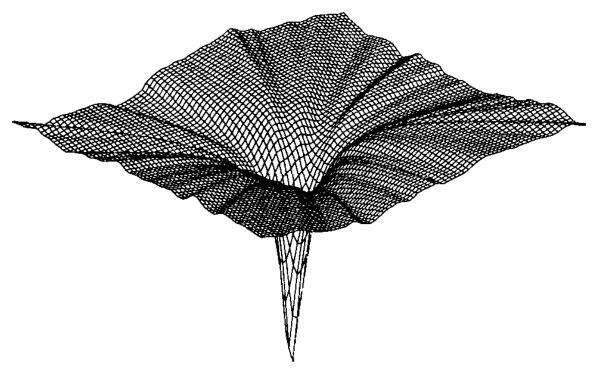
\includegraphics[width=\columnwidth]{fig23.png}
\caption{Example superficie ECM of sigmoide error.}\label{fig:23}
\end{figure}

\begin{figure}[t]
\centering
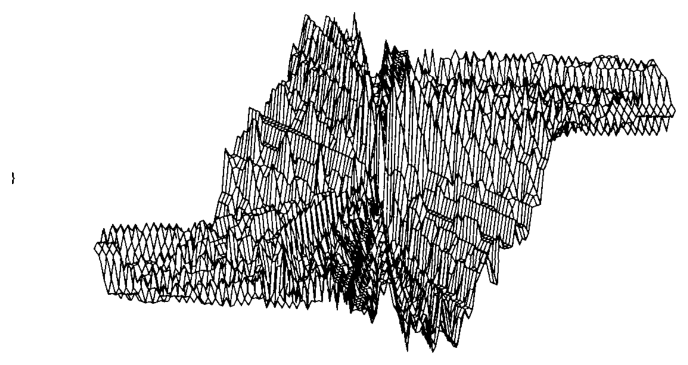
\includegraphics[width=\columnwidth]{fig24.png}
\caption{Example superficie ECM of signum error.}\label{fig:24}
\end{figure}

Although the above experiment is not all encompassing, we can infer from it that
minimizing the mean square of the error lineal is easy and minimizing the mean
square of the sigmoide error is more difficult, but typically much easier than
minimizing the mean square of the signum error. Only the error lineal is
guaranteed to have an superficie ECM with a unique mínimo global (assuming invertible
$\R$-matrix). Las otras superficies ECM pueden tener óptimos locales~\cite{sontag1,sontag2}.

In nonlinear neural networks, gradient methods generally work better with sigmoide
rather than signum nonlinearities. Smooth nonlinearities are required by the MRIII
and técnica de retropropagacións. Moreover, redes sigmoideales are capable of forming
representaciones internas that are more complex than simple binary codes and, thus,
these networks can often form decision regions that are more sophisticated than
those associated with similar redes signum. In fact, if a noiseless
infinite-precision Adaline sigmoideal could be constructed, it would be able to convey
an infinite amount of information at each time step. This is in contrast to the
maximum Shannon information capacity of one bit associated with each binary element.

The signum does have some advantages over the sigmoide in that it is easier to
implement in hardware and much simpler to compute on a computador digital.
Furthermore, the outputs of signums are binary signals which can be efficiently
manipulated by computadores digitales. In a red signum with binary inputs, for
instance, the output of each combinador lineal can be computed without performing
weight multiplications. This involves simply adding together the values of weights
with $+1$ inputs and subtracting from this the values of all weights that are
connected to $-1$ inputs.

A veces se usa un signum en una Adaline para producir decisiones de salida decisivas. The
probabilidad de error is then proportional to the mean square of the error de salida
$\tilde{\tilde{\epsilon}}$. To minimize this probabilidad de error approximately, one
can easily minimize $E[(\epsilon)^2]$ instead of directly minimizing
$E[(\tilde{\tilde{\epsilon}})^2]$~\cite{ieeewescon}. However, with only a little
more computation one could minimize $E[(\tilde{\epsilon})^2]$ and typically come
much closer to the objective of minimizing $E[(\tilde{\tilde{\epsilon}})^2]$. The
sigmoide can therefore be used in training the weights even when the signum is used
to form the Adaline output, as in Fig.~\ref{fig:21}.

%==============================================================================
\section{Steepest-Descent Rules---Multi-Element Networks}
%==============================================================================
We now study rules for descenso más pronunciado minimization of the MSE associated with
entire networks of Adaline sigmoideal elements. Like their mono-elemento
counterparts, the most practical and efficient descenso más pronunciado rules for
redes multi-elemento typically work with one pattern presentation at a time. We
will describe two descenso más pronunciado rules for multi-element redes sigmoideales,
retropropagación and Regla Madaline~III.

\subsection{Retropropagación for Networks}
The publication of the técnica de retropropagación by Rumelhart \textit{et
al.}~\cite{rhw86} has unquestionably been the most influential development in the
field of neural networks during the past decade. In retrospect, the technique
seems simple. Nonetheless, largely because early neural network research dealt
almost exclusively with de límite estricto nonlinearities, the idea never occurred to
neural network researchers throughout the 1960s.

Los conceptos básicos de la retropropagación se comprenden fácilmente. Unfortunately, these
simple ideas are often obscured by relatively intricate notation, so formal
derivations of the regla de retropropagación are often tedious. We present an informal
derivation of the algorithm and illustrate how it works for the simple network
shown in Fig.~\ref{fig:25}.

\begin{figure*}[t]
\centering
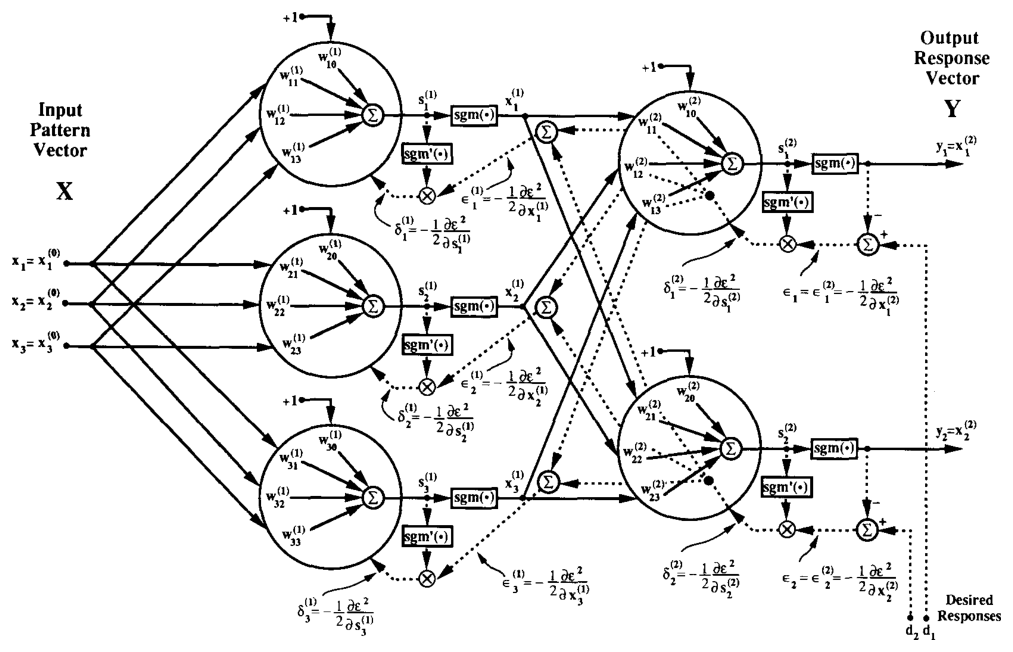
\includegraphics[width=0.92\textwidth]{fig25.png}
\caption{Example two-layer red de retropropagación architecture.}\label{fig:25}
\end{figure*}

The técnica de retropropagación is a nontrivial generalización of the single sigmoide
Adaline case of Section~VI-B. When applied to redes multi-elemento, the
técnica de retropropagación adjusts the weights in the direction opposite the
instantaneous error gradient:
\begin{equation}
\hat{\nabla}_k = \frac{\partial\epsilon_k^2}{\partial\W_k}
= \begin{bmatrix}\dfrac{\partial\epsilon_k^2}{\partial w_{1k}}\\[1.2ex]\vdots\\[0.6ex]\dfrac{\partial\epsilon_k^2}{\partial w_{mk}}\end{bmatrix}. \tag{68}
\end{equation}
Now, however, $\W_k$ is a long $m$-component vector of all weights in the entire
network. The instantaneous error cuadrático suma $\epsilon_k^2$ is the sum of the
squares of the errors at each of the $N_y$ outputs of the network. Thus
\begin{equation}
\epsilon_k^2 = \sum_{j=1}^{N_y}\epsilon_{jk}^2. \tag{69}
\end{equation}
In the network example shown in Fig.~\ref{fig:25}, the error cuadrático suma is given by
\begin{equation}
\epsilon^2 = (d_1 - y_1)^2 + (d_2 - y_2)^2 \tag{70}
\end{equation}
where we now suppress the time index $k$ for convenience.

In its simplest form, entrenamiento por retropropagación begins by presenting an input
vector de patrón $\X$ to the network, sweeping forward through the system to generate
an respuesta de salida vector $\bm{Y}$, and computing the errors at each output. The
next step involves sweeping the effects of the errors backward through the network
to associate a ``error cuadrático derivative'' $\delta$ with each Adaline, computing a
gradient from each $\delta$, and finally updating the weights of each Adaline based
upon the corresponding gradient. A new pattern is then presented and the process is
repeated. Los valores iniciales de los pesos normalmente se establecen en números aleatorios pequeños. The
algorithm will not work properly with redes multicapa if the pesos iniciales
are either zero or poorly chosen nonzero values.%
\footnote{Recently, Nguyen has discovered that a more sophisticated choice of
peso inicial values in capas ocultas can lead to reduced problems with local
optima and dramatic increases in network training speed~\cite{nguyen100}.
Experimental evidence suggests that it is advisable to choose the pesos iniciales
of each capa oculta in a quasi-random manner, which ensures that at each position
in a layer's input space the outputs of all but a few of its Adalines will be
saturated, while ensuring that each Adaline in the layer is unsaturated in some
region of its input space. When this method is used, the weights in the output
layer are set to small random values.}

We can get some idea about what is involved in the calculations associated with the
algoritmo de retropropagación by examining the network of Fig.~\ref{fig:25}. Each of
the five large circles represents a combinador lineal, as well as some associated
signal paths for error retropropagación, and the corresponding adaptive machinery
for updating the weights. This detail is shown in Fig.~\ref{fig:26}. The solid
lines in these diagrams represent forward signal paths through the network, and the
dotted lines represent the separate backward paths that are used in association
with calculations of the error cuadrático derivatives $\delta$. From Fig.~\ref{fig:25},
we see that the calculations associated with the barrido hacia atrás are of a complexity
roughly equal to that represented by the pasada hacia adelante through the network. The
barrido hacia atrás requires the same number of function calculations as the forward
sweep, but no weight multiplications in the first layer.

\begin{figure}[t]
\centering
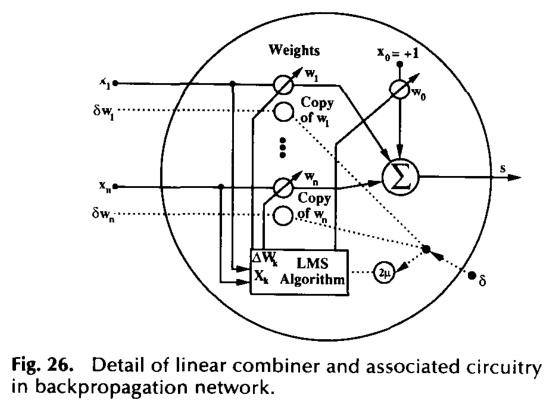
\includegraphics[width=\columnwidth]{fig26.png}
\caption{Detail of combinador lineal and associated circuitry in retropropagación
network.}\label{fig:26}
\end{figure}

As stated earlier, after a pattern has been presented to the network, and the
response error of each output has been calculated, the next step of the
algoritmo de retropropagación involves finding the instantaneous square-error
derivative $\delta$ associated with each punto de suma in the network. The
error cuadrático derivative associated with the $j$th Adaline in layer $l$ is defined
as%
\footnote{In Fig.~\ref{fig:25}, all notation follows the convention that
superscripts within parentheses indicate the layer number of the associated Adaline
or input node, while subscripts identify the associated Adaline(s) within a layer.}
\begin{equation}
\delta_j^{(l)} \triangleq -\frac{1}{2}\frac{\partial\epsilon^2}{\partial s_j^{(l)}}. \tag{71}
\end{equation}
Each of these derivatives in essence tells us how sensitive the sum square output
error of the network is to changes in the salida lineal of the associated Adaline
element.

The instantaneous square-error derivatives are first computed for each element in
the capa de salida. The calculation is simple. As an example, below we derive the
required expression for $\delta_1^{(2)}$, the derivative associated with the top
Adaline element in the capa de salida of Fig.~\ref{fig:25}. We begin with the
definition of $\delta_1^{(2)}$ from Eq.~(71)
\begin{equation}
\delta_1^{(2)} \triangleq -\frac{1}{2}\frac{\partial\epsilon^2}{\partial s_1^{(2)}}. \tag{72}
\end{equation}
Expanding the squared-error term $\epsilon^2$ by Eq.~(70) yields
\begin{align}
\delta_1^{(2)} &= -\frac{1}{2}\frac{\partial((d_1 - y_1)^2 + (d_2 - y_2)^2)}{\partial s_1^{(2)}} \tag{73}\\
&= -\frac{1}{2}\frac{\partial(d_1 - \sgm(s_1^{(2)}))^2}{\partial s_1^{(2)}}
   -\frac{1}{2}\frac{\partial(d_2 - \sgm(s_1^{(2)}))^2}{\partial s_1^{(2)}}. \tag{74}
\end{align}
We note that the second term is zero. Accordingly,
\begin{equation}
\delta_1^{(2)} = -\frac{1}{2}\frac{\partial(d_1 - \sgm(s_1^{(2)}))^2}{\partial s_1^{(2)}}. \tag{75}
\end{equation}
Observing that $d_1$ and $s_1^{(2)}$ are independent yields
\begin{align}
\delta_1^{(2)} &= -(d_1 - \sgm(s_1^{(2)}))\frac{\partial(-\sgm(s_1^{(2)}))}{\partial s_1^{(2)}} \tag{76}\\
&= (d_1 - \sgm(s_1^{(2)}))\,\sgm'(s_1^{(2)}). \tag{77}
\end{align}
We denote the error $d_1 - \sgm(s_1^{(2)})$, by $\epsilon_1^{(2)}$. Therefore,
\begin{equation}
\delta_1^{(2)} = \epsilon_1^{(2)}\,\sgm'(s_1^{(2)}). \tag{78}
\end{equation}
Note that this corresponds to the computation of $\delta_1^{(2)}$ as illustrated in
Fig.~\ref{fig:25}. The value of $\delta$ associated with the other output element
in the figure can be expressed in an analogous fashion. Thus each square-error
derivative $\delta$ in the capa de salida is computed by multiplying the error de salida
associated with that element by the derivative of the associated sigmoideal
nonlinearity. Note from Eq.~(55) that if the función sigmoidee is the hyperbolic
tangent, Eq.~(78) becomes simply
\begin{equation}
\delta_1^{(2)} = \epsilon_1^{(2)}(1 - (y_1)^2). \tag{79}
\end{equation}

Developing expressions for the square-error derivatives associated with hidden
layers is not much more difficult (refer to Fig.~\ref{fig:25}). We need an
expression for $\delta_1^{(1)}$, the square-error derivative associated with the top
element in the first layer of Fig.~\ref{fig:25}. The derivative $\delta_1^{(1)}$ is
defined by
\begin{equation}
\delta_1^{(1)} \triangleq -\frac{1}{2}\frac{\partial\epsilon^2}{\partial s_1^{(1)}}. \tag{80}
\end{equation}
Expanding this by the regla de la cadena, noting that $\epsilon^2$ is determined entirely by
the values of $s_1^{(2)}$ and $s_2^{(2)}$, yields
\begin{equation}
\delta_1^{(1)} = -\frac{1}{2}\!\left(\frac{\partial\epsilon^2}{\partial s_1^{(2)}}\frac{\partial s_1^{(2)}}{\partial s_1^{(1)}}
+ \frac{\partial\epsilon^2}{\partial s_2^{(2)}}\frac{\partial s_2^{(2)}}{\partial s_1^{(1)}}\right). \tag{81}
\end{equation}
Using the definitions of $\delta_1^{(2)}$ and $\delta_2^{(2)}$, and then
substituting expanded versions of Adaline salida lineals $s_1^{(2)}$ and
$s_2^{(2)}$ gives
\begin{align}
\delta_1^{(1)} &= \delta_1^{(2)}\frac{\partial s_1^{(2)}}{\partial s_1^{(1)}}
+ \delta_2^{(2)}\frac{\partial s_2^{(2)}}{\partial s_1^{(1)}} \tag{82}\\
&= \delta_1^{(2)}\frac{\partial}{\partial s_1^{(1)}}\!\left(w_{10}^{(2)} + \sum_{i=1}^{3}w_{1i}^{(2)}\sgm(s_i^{(1)})\right)\notag\\
&\quad + \delta_2^{(2)}\frac{\partial}{\partial s_1^{(1)}}\!\left(w_{20}^{(2)} + \sum_{i=1}^{3}w_{2i}^{(2)}\sgm(s_i^{(1)})\right). \tag{83}
\end{align}
Noting that $\partial[\sgm(s_i^{(1)})]/\partial s_1^{(1)} = 0$, $i \neq j$, leaves
\begin{align}
\delta_1^{(1)} &= \delta_1^{(2)}w_{11}^{(2)}\sgm'(s_1^{(1)}) + \delta_2^{(2)}w_{21}^{(2)}\sgm'(s_1^{(1)}) \tag{84}\\
&= [\delta_1^{(2)}w_{11}^{(2)} + \delta_2^{(2)}w_{21}^{(2)}]\,\sgm'(s_1^{(1)}). \tag{85}
\end{align}
Now, we make the following definition:
\begin{equation}
\epsilon_1^{(1)} \triangleq \delta_1^{(2)}w_{11}^{(2)} + \delta_2^{(2)}w_{21}^{(2)}. \tag{86}
\end{equation}
Accordingly,
\begin{equation}
\delta_1^{(1)} = \epsilon_1^{(1)}\,\sgm'(s_1^{(1)}). \tag{87}
\end{equation}
Referring to Fig.~\ref{fig:25}, we can trace through the circuit to verify that
$\delta_1^{(1)}$ is computed in accord with Eqs.~(86) and~(87).

The easiest way to find values of $\delta$ for all the Adaline elements in the
network is to follow the schematic diagram of Fig.~\ref{fig:25}.

Thus, the procedure for finding $\delta^{(l)}$, the square-error derivative
associated with a given Adaline in capa oculta $l$, involves respectively
multiplying each derivative $\delta^{(l+1)}$ associated with each element in the
layer immediately downstream from a given Adaline by the weight that connects it to
the given Adaline. These weighted square-error derivatives are then added together,
producing an error term $\epsilon^{(l)}$, which, in turn, is multiplied by
$\sgm'(s^{(l)})$, the derivative of the given Adaline's función sigmoidee at its
current punto de operación. If a network has more than two layers, this process of
backpropagating the instantaneous square-error derivatives from one layer to the
immediately preceding layer is successively repeated until a square-error
derivative $\delta$ is computed for each Adaline in the network. This is easily
shown at each layer by repeating the regla de la cadena argument associated with Eq.~(81).

We now have a general method for finding a derivative $\delta$ for each Adaline
element in the network. The next step is to use these $\delta$'s to obtain the
corresponding gradients. Consider an Adaline somewhere in the network which, during
presentation $k$, has a vector de pesos $\W_k$, an vector de entrada $\X_k$, and a linear
output $s_k = \W_k^{T}\X_k$. The gradiente instantáneo for this Adaline element is
\begin{equation}
\hat{\nabla}_k = \frac{\partial\epsilon_k^2}{\partial\W_k}. \tag{88}
\end{equation}
This can be written as
\begin{equation}
\hat{\nabla}_k = \frac{\partial\epsilon_k^2}{\partial\W_k}
= \frac{\partial\epsilon_k^2}{\partial s_k}\frac{\partial s_k}{\partial\W_k}. \tag{89}
\end{equation}
Note that $\W_k$ and $\X_k$ are independent so
\begin{equation}
\frac{\partial s_k}{\partial\W_k} = \frac{\partial\W_k^{T}\X_k}{\partial\W_k} = \X_k. \tag{90}
\end{equation}
Therefore,
\begin{equation}
\hat{\nabla}_k = \frac{\partial\epsilon_k^2}{\partial s_k}\X_k. \tag{91}
\end{equation}
For this element,
\begin{equation}
\delta_k = -\frac{1}{2}\frac{\partial\epsilon_k^2}{\partial s_k}. \tag{92}
\end{equation}
Accordingly,
\begin{equation}
\hat{\nabla}_k = -2\delta_k\X_k. \tag{93}
\end{equation}
Updating the weights of the Adaline element using the method of descenso más pronunciado
with the gradiente instantáneo is a process represented by
\begin{equation}
\W_{k+1} = \W_k + \mu(-\hat{\nabla}_k) = \W_k + 2\mu\delta_k\X_k. \tag{94}
\end{equation}
Thus, after backpropagating all square-error derivatives, we complete a
retropropagación iteration by adding to each vector de pesos the corresponding input
vector scaled by the associated square-error derivative. Eq.~(94) and the means for
finding $\delta_k$ comprise the general actualización de pesos rule of the retropropagación
algorithm.

There is a great similarity between Eq.~(94) and the $\mu$-algoritmo LMS~(33), but
one should view this similarity with caution. The quantity $\delta_k$, defined as a
squared-error derivative, might appear to play the same role in retropropagación as
that played by the error in the $\mu$-algoritmo LMS. However, $\delta_k$ is not an
error. Adaptation of the given Adaline is effected to reduce the squared output
error $\epsilon_k^2$, not $\delta_k$ of the given Adaline or of any other Adaline in
the network. The objective is not to reduce the $\delta_k$'s of the network, but to
reduce $\epsilon_k^2$ at the network output.

It is interesting to examine the actualización de pesoss that retropropagación imposes on the
Adaline elements in the capa de salida. Substituting Eq.~(77) into Eq.~(94) reveals
the Adaline which provides output $y_1$ in Fig.~\ref{fig:25} is updated by the rule
\begin{equation}
\W_{k+1} = \W_k + 2\mu\epsilon_1^{(2)}\,\sgm'(s_1^{(2)})\X_k. \tag{95}
\end{equation}
This rule turns out to be identical to the single Adaline version~(54) of the
regla de retropropagación. This is not surprising since the output Adaline is provided
with both input signals and respuestas deseadas, so its training circumstance is the
same as that experienced by an Adaline trained in isolation.

There are many variants of the algoritmo de retropropagación. Sometimes, the size of
$\mu$ is reduced during training to diminish the effects of ruido de gradiente in the
weights. Another extension is the técnica de momento~\cite{rhw86} which involves
including in the cambio de pesos vector $\Delta\W_k$ of each Adaline a term
proportional to the corresponding cambio de pesos from the previous iteration. That
is, Eq.~(94) is replaced by a pair of equations:
\begin{align}
\Delta\W_k &= 2\mu(1-\eta)\delta_k\X_k + \eta\Delta\W_{k-1} \tag{96}\\
\W_{k+1} &= \W_k + \Delta\W_k. \tag{97}
\end{align}
where the constante de momento $0 \le \eta < 1$ is in practice usually set to
something around 0.8 or 0.9.

The técnica de momento filtros pasa-bajos the actualización de pesoss and thereby tends to
resist erratic cambios de pesos caused either by ruido de gradiente or high spatial
frequencies in the superficie ECM. The factor $(1-\eta)$ in Eq.~(96) is included to
give the filter a ganancia DC of unity so that the tasa de aprendizaje $\mu$ does not need to
be stepped down as the constante de momento $\eta$ is increased. A momentum term can
also be added to the update equations of other algorithms discussed in this paper.
A detailed analysis of stability issues associated with momentum updating for the
$\mu$-algoritmo LMS, for instance, has been described by Shynk and Roy~\cite{shynk}.

In our experience, the técnica de momento used alone is usually of little value. We
have found, however, that it is often useful to apply the technique in situations
that require relatively ``clean''%
\footnote{``Clean'' estimación del gradientes are those with little ruido de gradiente.}
estimación del gradientes. One case is a normalized actualización de pesos equation which makes the
network's vector de pesos move the same distancia euclidiana with each iteration. This
can be accomplished by replacing Eq.~(96) and~(97) with
\begin{align}
\Delta_k &= \delta_k\X_k + \eta\Delta_{k+1} \tag{98}\\
\W_{k+1} &= \W_k + \frac{\mu\Delta_k}{\sqrt{\displaystyle\sum_{\text{all Adalines}}|\Delta_k|^2}}. \tag{99}
\end{align}
where again $0 < \eta < 1$. The actualización de pesoss determined by Eqs.~(98) and~(99) can
help a network find a solution when a relatively flat local region in the MSE
surface is encountered. The weights move by the same amount whether the surface is
flat or inclined. It is reminiscent of $\alpha$-LMS because the gradient term in the
actualización de pesos equation is normalized by a time-varying factor. The actualización de pesos
rule could be further modified by including terms from both techniques associated
with Eqs.~(96) through~(99). Other methods for speeding up entrenamiento por retropropagación
include Fahlman's popular quickprop method~\cite{fahlman}, as well as the
delta-bar-delta approach reported in an excellent paper by Jacobs~\cite{jacobs}.%
\footnote{Jacob's paper, like many other papers in the literature, assumes for
analysis that the gradiente verdaderos rather than gradiente instantáneos are used to
update the weights, that is, that weights are changed periodically, only after all
patrones de entrenamiento are presented. This eliminates ruido de gradiente but can slow down
training enormously if the conjunto de entrenamiento is large. The delta-bar-delta procedure in
Jacob's paper involves monitoring changes of the gradiente verdaderos in response to
cambios de pesos. It should be possible to avoid the expense of computing the true
gradients explicitly in this case by instead monitoring changes in the outputs of,
say, two momentum filters with different time constants.}

One of the most promising new areas of neural network research involves
retropropagación variants for training various recurrent (retroalimentación de señal)
networks. Recently, regla de retropropagacións have been derived for training recurrent
networks to learn static associations~\cite{pineda,almeida}. More interesting is
the on-line technique of Williams and Zipser~\cite{williams} which allows a wide
class of redes recurrentes to learn dynamic associations and trajectories. A more
general and computationally viable variant of this technique has been advanced by
Narendra and Parthasarathy~\cite{narendra}. These on-line methods are
generalizacións of a well-known descenso más pronunciado algorithm for training linear IIR
filters~\cite{white,asp}.

An equivalent technique that is usually far less computationally intensive but best
suited for off-line computation~\cite{werbos,rhw86,pearlmutter}, called
``retropropagación through time,'' has been used by Nguyen and Widrow~\cite{nguyen90}
to enable a neural network to learn without a teacher how to back up a
computer-simulated camión con remolque to a plataforma de carga (Fig.~\ref{fig:27}). This is a
highly dirección no lineal task and it is not yet known how to design a controller to
perform it. Nevertheless, with just 6 inputs providing information about the current
position of the truck, a two-layer neural network with only 26 Adalines was able to
learn of its own accord to solve this problem. Once trained, the network could
successfully back up the truck from any initial position and orientation in front of
the plataforma de carga.

\begin{figure}[t]
\centering
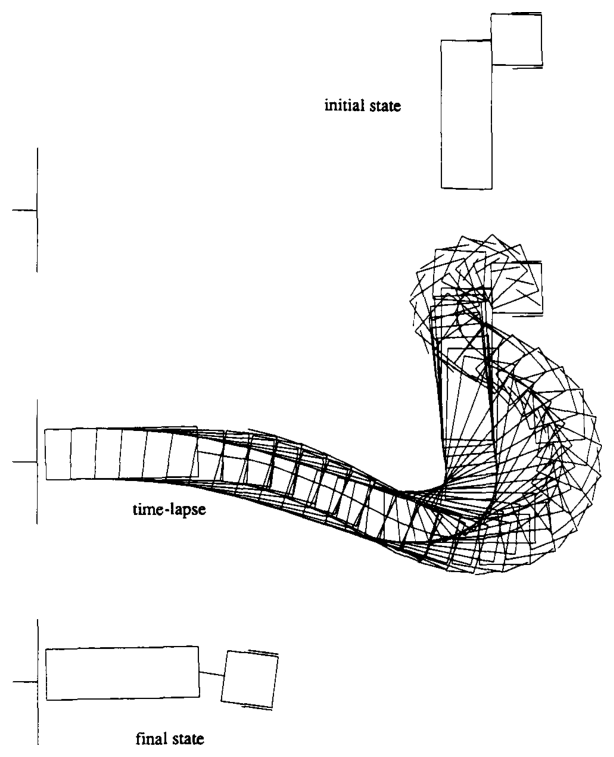
\includegraphics[width=0.9\columnwidth]{fig27.png}
\caption{Example truck backup sequence.}\label{fig:27}
\end{figure}

\subsection{Regla Madaline III for Networks}
It is difficult to build neural networks with hardware analógico that can be trained
effectively by the popular técnica de retropropagación. Attempts to overcome this
difficulty have led to the development of the MRIII algorithm. A commercial analog
neurocomputing chip based primarily on this algorithm has already been
devised~\cite{holler}. The method described in this section is a generalización of
the single Adaline MRIII technique~(60). The multi-element generalización of the
other single element MRIII rule~(61) is described in~\cite{mriii}.

\begin{figure}[t]
\centering
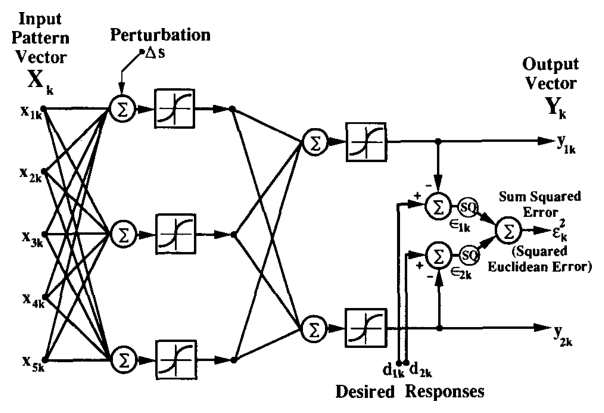
\includegraphics[width=\columnwidth]{fig28.png}
\caption{Example two-layer Madaline~III architecture.}\label{fig:28}
\end{figure}

The MRIII algorithm can be readily described by referring to Fig.~\ref{fig:28}.
Although this figure shows a simple two-layer feedforward architecture, the
procedure to be developed will work for neural networks with any number of Adaline
elements in any feedforward structure. In~\cite{mriii}, we discuss variants of the
basic MRIII approach that allow descenso más pronunciado training to be applied to more
general network topologies, even those with retroalimentación de señal.

Assume that an patrón de entrada $\X$ and its associated desired respuestas de salida $d_1$
and $d_2$ are presented to the network of Fig.~\ref{fig:28}. At this point, we
measure the sum squared respuesta de salida error $\epsilon^2 = (d_1 - y_1)^2 + (d_2 -
y_2)^2 = \epsilon_1^2 + \epsilon_2^2$. We then add a small quantity $\Delta s$ to a
selected Adaline in the network, providing a perturbation to the element's linear
sum. This perturbation propagates through the network, and causes a change in the
sum of the squares of the errors, $\Delta(\epsilon^2) = \Delta(\epsilon_1^2 +
\epsilon_2^2)$. An easily measured ratio is
\begin{equation}
\frac{\Delta(\epsilon^2)}{\Delta s} = \frac{\Delta(\epsilon_1^2 + \epsilon_2^2)}{\Delta s}
\simeq \frac{\partial(\epsilon^2)}{\partial s}. \tag{100}
\end{equation}
Below we use this to obtain the gradiente instantáneo of $\epsilon_k^2$ with respect
to the vector de pesos of the selected Adaline. For the $k$th presentation, the
gradiente instantáneo is
\begin{equation}
\hat{\nabla}_k = \frac{\partial(\epsilon_k^2)}{\partial\W_k}
= \frac{\partial(\epsilon_k^2)}{\partial s_k}\frac{\partial s_k}{\partial\W_k}
= \frac{\partial(\epsilon_k^2)}{\partial s_k}\X_k. \tag{101}
\end{equation}
Replacing the derivative with a ratio of differences yields
\begin{equation}
\hat{\nabla}_k \simeq \frac{\Delta(\epsilon_k^2)}{\Delta s}\X_k. \tag{102}
\end{equation}
The idea of obtaining a derivative by perturbing the salida lineal of the selected
Adaline element is the same as that expressed for the single element in
Section~VI-B, except that here the error is obtained from the output of a
red multi-elemento rather than from the output of a single element.

The gradient~(102) can be used to optimize the vector de pesos in accord with the
method of descenso más pronunciado:
\begin{equation}
\W_{k+1} = \W_k - \mu\frac{\Delta(\epsilon_k^2)}{\Delta s}\X_k. \tag{103}
\end{equation}
Maintaining the same patrón de entrada, one could either perturb all the elements in the
network in sequence, adapting after each gradient calculation, or else the
derivatives could be computed and stored to allow all Adalines to be adapted at
once. These two MRIII approaches both involve the same actualización de pesos equation~(103),
and if $\mu$ is small, both lead to equivalent solutions. With large $\mu$,
experience indicates that adapting one element at a time results in convergence
after fewer iterations, especially in large networks. Storing the gradients,
however, has the advantage that after the initial unperturbed error is measured
during a given training presentation, each estimación del gradiente requires only the
perturbed error measurement. If adaptations take place after each error measurement,
both perturbed and unperturbed errors must be measured for each gradient
calculation. This is because each actualización de pesos changes the associated unperturbed
error.

\subsection{Comparison of MRIII with MRII}
MRIII se derivó de MRII reemplazando las no linealidades signum por sigmoidees.
The similarity of these algorithms becomes evident when comparing Fig.~\ref{fig:28},
representing MRIII, with Fig.~\ref{fig:16}, representing MRII.

La red MRII es altamente discontinua y no lineal. Using an instantaneous
gradient to adjust the weights is not possible. In fact, from the superficie ECM for
the Adaline signum presented in Section~VI-B, it is clear that even descenso por gradiente
techniques that use the gradiente verdadero could run into severe problems with local
minima. The idea of adding a perturbation to the linear sum of a selected Adaline
element is workable, however. If the error de Hamming has been reduced by the
perturbation, the Adaline is adapted to reverse its decisión de salida. This weight
change is in the LMS direction, along its $\X$-vector. If adapting the Adaline would
not reduce network error de salida, it is not adapted. This is in accord with the
principio de mínima perturbación. The Adalines selected for possible adaptation are
those whose analog sums are closest to zero, that is, the Adalines that can be
adapted to give opposite responses with the smallest cambios de pesos. It is useful to
note that with binary $\pm 1$ desired responses, the Hamming error is equal to
$1/4$ the error cuadrático suma. Minimizing the error de salida de Hamming is therefore
equivalent to minimizing the error de salida cuadrático suma.

El algoritmo MRIII funciona de manera similar. All the Adalines in the MRIII network
are adapted, but those whose analog sums are closest to zero will usually be adapted
most strongly, because the sigmoide has its maximum slope at zero, contributing to
high gradient values. As with MRII, the objective is to change the weights for the
given input presentation to reduce the error cuadrático suma at the network output. In
accord with the principio de mínima perturbación, the vectores de pesos of the Adaline
elements are adapted in the LMS direction, along their $\X$-vectors, and are adapted
in proportion to their capabilities for reducing the error cuadrático suma (the square of
the error euclidiano) at the output.

\subsection{Comparison of MRIII with Retropropagación}
In Section~VI-B, we argued that for the Adaline sigmoideal element, the MRIII
algorithm~(61) is essentially equivalent to the algoritmo de retropropagación~(54). The
same argument can be extended to the network of Adaline elements, demonstrating that
if $\Delta s$ is small and adaptation is applied to all elements in the network at
once, then MRIII is essentially equivalent to retropropagación. That is, to the
extent that the sample derivative $\Delta\epsilon_k^2/\Delta s$ from Eq.~(103) is
equal to the analytical derivative $\partial\epsilon_k^2/\partial s_k$ from Eq.~(91),
the two rules follow identical gradiente instantáneos, and thus perform identical
actualización de pesoss.

The algoritmo de retropropagación requires fewer operations than MRIII to calculate
gradients, since it is able to take advantage of \textit{a priori} knowledge of the
sigmoide nonlinearities and their derivative functions. Conversely, the MRIII
algorithm uses no prior knowledge about the characteristics of the sigmoide
functions. Rather, it acquires gradiente instantáneos from perturbation
measurements. Using MRIII, tolerances on the sigmoide implementations can be greatly
relaxed compared to acceptable tolerances for successful retropropagación.

Steepest-descent training of redes multicapa implemented by computer simulation
or by precise parallel digital hardware is usually best carried out by
retropropagación. During each training presentation, the retropropagación method
requires only one forward computation through the network followed by one backward
computation in order to adapt all the weights of an entire network. To accomplish
the same effect with the form of MRIII that updates all weights at once, one
measures the unperturbed error followed by a number of perturbed error measurements
equal to the number of elements in the network. This could require a lot of
computation.

If a network is to be implemented in hardware analógico, however, experience has shown
that MRIII offers strong advantages over retropropagación. Comparison of
Fig.~\ref{fig:25} with Fig.~\ref{fig:28} demonstrates the relative simplicity of
MRIII. All the apparatus for backward propagation of error-related signals is
eliminated, and the weights do not need to carry signals in both directions (see
Fig.~\ref{fig:26}). MRIII is a much simpler algorithm to build and to understand,
and in principle it produces the same gradiente instantáneo as the retropropagación
algorithm. The técnica de momento and most other common variants of the
algoritmo de retropropagación can be applied to MRIII training.

\subsection{MSE Surfaces of Neural Networks}
In Section~VI-B, ``typical'' mean-square-error surfaces of sigmoide and signum
Adalines were shown, indicating that Adaline sigmoideals are much more conducive to
gradient approaches than Adaline signums. The same phenomena result when Adalines
are incorporated into redes multi-elemento. The superficies ECM of MRII networks are
reasonably chaotic and will not be explored here. In this section we examine only
superficies ECM from a typical entrenamiento por retropropagación problem with a sigmoideal neural
network.

In a network with more than two weights, the superficie ECM is high-dimensional and
difficult to visualize. It is possible, however, to look at slices of this surface
by plotting the superficie ECM created by varying two of the weights while holding all
others constant. The surfaces plotted in Figs.~\ref{fig:29} and~\ref{fig:30} show
two such slices of the superficie ECM from a typical learning problem involving,
respectively, an untrained sigmoideal network and a trained one. The first surface
resulted from varying two de la primera capa weights of an untrained network. The second
surface resulted from varying the same two weights after the network was fully
trained. The two surfaces are similar, but the second one has a deeper minimum which
was carved out by the retropropagación learning process. Figs.~\ref{fig:31}
and~\ref{fig:32} resulted from varying a different set of two weights in the same
network. Fig.~\ref{fig:31} is the result from varying a de la primera capa weight and
de la tercera capa weight in the untrained network, whereas Fig.~\ref{fig:32} is the
surface that resulted from varying the same two weights after the network was
trained.

\begin{figure}[t]
\centering
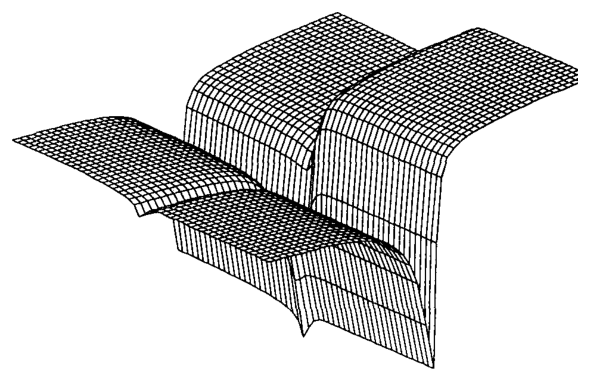
\includegraphics[width=\columnwidth]{fig29.png}
\caption{Example superficie ECM of untrained sigmoideal network as a function of two
de la primera capa weights.}\label{fig:29}
\end{figure}

\begin{figure}[t]
\centering
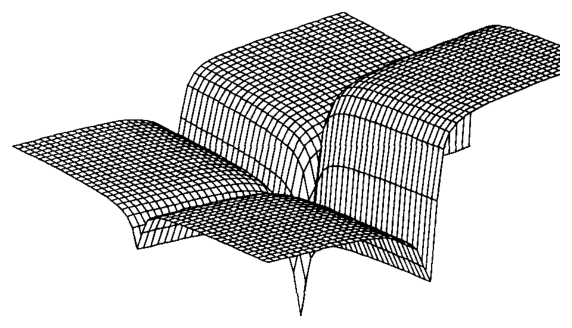
\includegraphics[width=\columnwidth]{fig30.png}
\caption{Example superficie ECM of trained sigmoideal network as a function of two
de la primera capa weights.}\label{fig:30}
\end{figure}

\begin{figure}[t]
\centering
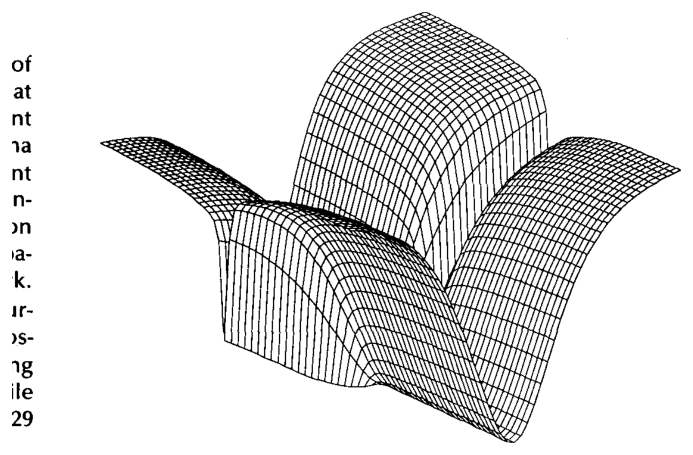
\includegraphics[width=\columnwidth]{fig31.png}
\caption{Example superficie ECM of untrained sigmoideal network as a function of a
de la primera capa weight and a de la tercera capa weight.}\label{fig:31}
\end{figure}

\begin{figure}[t]
\centering
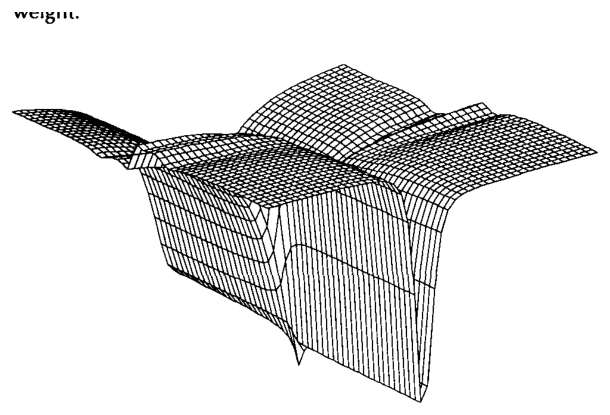
\includegraphics[width=\columnwidth]{fig32.png}
\caption{Example superficie ECM of trained sigmoideal network as a function of a
de la primera capa weight and a de la tercera capa weight.}\label{fig:32}
\end{figure}

By studying many plots, it becomes clear that retropropagación and MRIII will be
subject to convergence on óptimos locales. Lo mismo es cierto para MRII. The most common
remedy for this is the sporadic addition of noise to the weights or gradients. Some
of the ``recocido simulado'' methods~\cite{pdp} do this. Another method involves
retraining the network several times using different random peso inicial values
until a satisfactory solution is found.

Solutions found by people in everyday life are usually not optimal, but many of them
are useful. If a local optimum yields satisfactory performance, often there is
simply no need to search for a better solution.

%==============================================================================
\section{Summary}
%==============================================================================
This year is the 30th anniversary of the publication of the regla del Perceptrón by
Rosenblatt and the algoritmo LMS by Widrow and Hoff. It has also been 16 years since
Werbos first published the algoritmo de retropropagación. These reglas de aprendizaje and
several others have been studied and compared. Although they differ significantly
from each other, they all belong to the same ``family.''

Se estableció una distinción entre reglas de corrección de error y reglas de descenso más pronunciado.
The former includes the regla del Perceptrón, Mays' rules, the $\alpha$-algoritmo LMS,
the original Madaline~I rule of 1962, and the Madaline~II rule. The latter includes
the $\mu$-algoritmo LMS, the Madaline~III rule, and the algoritmo de retropropagación.
Fig.~\ref{fig:33} categorizes the reglas de aprendizaje that have been studied.

\begin{figure}[t]
\centering
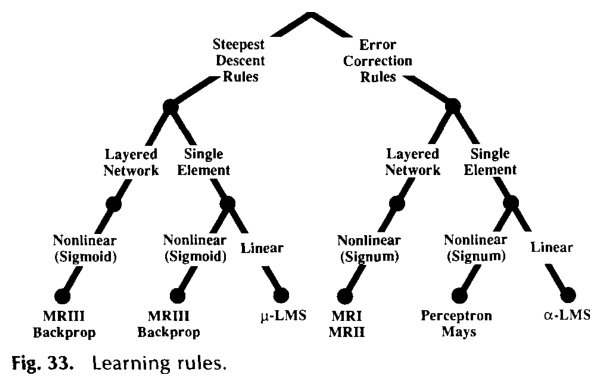
\includegraphics[width=\columnwidth]{fig33.png}
\caption{Learning rules.}\label{fig:33}
\end{figure}

Although these algorithms have been presented as established reglas de aprendizaje, one
should not gain the impression that they are perfect and frozen for all time.
Son posibles variaciones para cada uno de ellos. They should be regarded as substrates
upon which to build new and better rules. There is a tremendous amount of invention
waiting ``in the wings.'' Esperamos con interés los próximos 30 años.

%==============================================================================
\begin{thebibliography}{133}
\small
\bibitem{steinbuch} K. Steinbuch and V. A. W. Piske, ``Learning matrices and their applications,'' \textit{IEEE Trans. Electron. Comput.}, vol. EC-12, pp. 846--862, Dec. 1963.
\bibitem{widrow62} B. Widrow, ``Generalization and information storage in networks of adaline `neurons','' in \textit{Self-Organizing Systems 1962}, M. Yovitz, G. Jacobi, and G. Goldstein, Eds. Washington, DC: Spartan Books, 1962, pp. 435--461.
\bibitem{stark} L. Stark, M. Okajima, and G. H. Whipple, ``Computer reconocimiento de patrones techniques: Electrocardiographic diagnosis,'' \textit{Commun. Ass. Comput. Mach.}, vol. 5, pp. 527--532, Oct. 1962.
\bibitem{rosen58} F. Rosenblatt, ``Two theorems of statistical separability in the perceptron,'' in \textit{Mechanization of Thought Processes: Proc. Symp. National Physical Laboratory, Nov. 1958}, vol. 1, pp. 421--456. London: HM Stationery Office, 1959.
\bibitem{rosen62} F. Rosenblatt, \textit{Principles of Neurodynamics: Perceptróns and the Theory of Brain Mechanisms}. Washington, DC: Spartan Books, 1962.
\bibitem{malsburg} C. von der Malsburg, ``Self-organizing of orientation sensitive cells in the striate cortex,'' \textit{Kybernetik}, vol. 14, pp. 85--100, 1973.
\bibitem{gross76a} S. Grossberg, ``Adaptive pattern classification and universal recoding, I: Parallel development and coding of neural detectores de características,'' \textit{Biolog. Cybernetics}, vol. 23, pp. 121--134, 1976.
\bibitem{fuku75} K. Fukushima, ``Cognitrón: A autoorganizado multilayered neural network,'' \textit{Biolog. Cybernetics}, vol. 20, pp. 121--136, 1975.
\bibitem{fuku80} K. Fukushima, ``Neocognitrón: A autoorganizado neural network model for a mechanism of reconocimiento de patrones unaffected by shift in position,'' \textit{Biolog. Cybernetics}, vol. 36, pp. 193--202, 1980.
\bibitem{boot66} B. Widrow, ``Bootstrap learning in lógica de umbral systems,'' presented at the American Automatic Control Council (Theory Committee), IFAC Meeting, London, England, June 1966.
\bibitem{boot73} B. Widrow, N. K. Gupta, and S. Maitra, ``Punish/reward: Learning with a critic in adaptive threshold systems,'' \textit{IEEE Trans. Syst., Man, Cybernetics}, vol. SMC-3, pp. 455--465, Sept. 1973.
\bibitem{barto} A. G. Barto, R. S. Sutton, and C. W. Anderson, ``Neuronlike adaptive elements that can solve difficult learning control problems,'' \textit{IEEE Trans. Syst., Man, Cybernetics}, vol. SMC-13, pp. 834--846, 1983.
\bibitem{albus} J. S. Albus, ``A new approach to manipulator control: the cerebellar model articulation controller (CMAC),'' \textit{J. Dyn. Sys., Meas., Contr.}, vol. 97, pp. 220--227, 1975.
\bibitem{miller} W. T. Miller, III, ``Sensor-based control of robotic manipulators using a general algoritmo de aprendizaje,'' \textit{IEEE J. Robotics Automat.}, vol. RA-3, pp. 157--165, Apr. 1987.
\bibitem{gross76b} S. Grossberg, ``Adaptive pattern classification and universal recoding, II: Feedback, expectation, olfaction, and illusions,'' \textit{Biolog. Cybernetics}, vol. 23, pp. 187--202, 1976.
\bibitem{art1} G. A. Carpenter and S. Grossberg, ``A massively parallel architecture for a autoorganizado neural reconocimiento de patrones machine,'' \textit{Computer Vision, Graphics, and Image Processing}, vol. 37, pp. 54--115, 1983.
\bibitem{art2} G. A. Carpenter and S. Grossberg, ``Art 2: Self-organization of stable category recognition codes for analog output patterns,'' \textit{Applied Optics}, vol. 26, pp. 4919--4930, Dec. 1, 1987.
\bibitem{art3} G. A. Carpenter and S. Grossberg, ``Art 3 hierarchical search: Chemical transmitters in autoorganizado reconocimiento de patrones architectures,'' in \textit{Proc. Int. Joint Conf. on Neural Networks}, vol. 2, pp. 30--33, Wash., DC, Jan. 1990.
\bibitem{koh82} T. Kohonen, ``Self-organized formation of topologically correct mapas de características,'' \textit{Biolog. Cybernetics}, vol. 43, pp. 59--69, 1982.
\bibitem{koh88} T. Kohonen, \textit{Self-organization and Associative Memory}. New York: Springer-Verlag, 2d ed., 1988.
\bibitem{hebb} D. O. Hebb, \textit{The Organization of Behavior}. New York: Wiley, 1949.
\bibitem{hop82} J. J. Hopfield, ``Neural networks and physical systems with emergent collective computational abilities,'' \textit{Proc. Natl. Acad. Sci.}, vol. 79, pp. 2554--2558, Apr. 1982.
\bibitem{hop84} J. J. Hopfield, ``Neurons with graded response have collective computational properties like those of two-state neurons,'' \textit{Proc. Natl. Acad. Sci.}, vol. 81, pp. 3088--3092, May 1984.
\bibitem{kosko} B. Kosko, ``Adaptive bidirectional associative memories,'' \textit{Appl. Optics}, vol. 26, pp. 4947--4960, Dec. 1, 1987.
\bibitem{boltz1} G. E. Hinton, R. J. Sejnowski, and D. H. Ackley, ``Boltzmann machines: Constraint satisfaction networks that learn,'' Tech. Rep. CMU-CS-84-119, Carnegie-Mellon University, Dept. of Computer Science, 1984.
\bibitem{boltz2} G. E. Hinton and T. J. Sejnowski, ``Learning and relearning in Boltzmann machines,'' in \textit{Parallel Distributed Processing}, vol. 1, ch. 7, D. E. Rumelhart and J. L. McClelland, Eds. Cambridge, MA: M.I.T. Press, 1986.
\bibitem{talbert} L. R. Talbert \textit{et al.}, ``A real-time adaptive speech-recognition system,'' Tech. rep., Stanford University, 1963.
\bibitem{hu} M. J. C. Hu, \textit{Application of the Adaline System to Weather Forecasting}. Thesis, Tech. Rep. 6775-1, Stanford Electron. Labs., Stanford, CA, June 1964.
\bibitem{broom} B. Widrow, ``The original adaptive neural net broom-balancer,'' \textit{Proc. IEEE Intl. Symp. Circuits and Systems}, pp. 351--357, Phila., PA, May 4--7 1987.
\bibitem{asp} B. Widrow and S. D. Stearns, \textit{Adaptive Signal Processing}. Englewood Cliffs, NJ: Prentice-Hall, 1985.
\bibitem{antenna} B. Widrow, P. Mantey, L. Griffiths, and B. Goode, ``Adaptive antenna systems,'' \textit{Proc. IEEE}, vol. 55, pp. 2143--2159, Dec. 1967.
\bibitem{invctrl} B. Widrow, ``Adaptive inverse control,'' \textit{Proc. 2d Intl. Fed. of Automatic Control Workshop}, pp. 1--5, Lund, Sweden, July 1--3, 1986.
\bibitem{anc} B. Widrow \textit{et al.}, ``Adaptive noise cancelling: Principles and applications,'' \textit{Proc. IEEE}, vol. 63, pp. 1692--1716, Dec. 1975.
\bibitem{lucky1} R. W. Lucky, ``Automatic equalization for digital communication,'' \textit{Bell Syst. Tech. J.}, vol. 44, pp. 547--588, Apr. 1965.
\bibitem{lucky2} R. W. Lucky \textit{et al.}, \textit{Principles of Data Communication}. New York: McGraw-Hill, 1968.
\bibitem{sondhi} M. M. Sondhi, ``An cancelador de eco adaptativo,'' \textit{Bell Syst. Tech. J.}, vol. 46, pp. 497--511, Mar. 1967.
\bibitem{werbos} P. Werbos, \textit{Beyond Regression: New Tools for Prediction and Analysis in the Behavioral Sciences}. tesis doctoral, Harvard University, Cambridge, MA, Aug. 1974.
\bibitem{lecun} Y. le Cun, ``A theoretical framework for back-propagation,'' in \textit{Proc. 1988 Connectionist Models Summer School}, D. Touretzky, G. Hinton, and T. Sejnowski, Eds. June 17--26, pp. 21--28. San Mateo, CA: Morgan Kaufmann.
\bibitem{parker82} D. Parker, ``Learning-logic,'' Invention Report S81-64, File 1, Office of Technology Licensing, Stanford University, Stanford, CA, Oct. 1982.
\bibitem{parker85} D. Parker, ``Learning-logic,'' Technical Report TR-47, Center for Computational Research in Economics and Management Science, M.I.T., Apr. 1985.
\bibitem{rhw85} D. E. Rumelhart, G. E. Hinton, and R. J. Williams, ``Learning representaciones internas by error propagation,'' ICS Report 8506, Institute for Cognitive Science, UCSD, La Jolla, CA, Sept. 1985.
\bibitem{rhw86} D. E. Rumelhart, G. E. Hinton, and R. J. Williams, ``Learning representaciones internas by error propagation,'' in \textit{Parallel Distributed Processing}, vol. 1, ch. 8, D. E. Rumelhart and J. L. McClelland, Eds. Cambridge, MA: M.I.T. Press, 1986.
\bibitem{wwb} B. Widrow, R. G. Winter, and R. Baxter, ``Learning phenomena in layered neural networks,'' \textit{Proc. 1st IEEE Intl. Conf. on Neural Networks}, vol. 2, pp. 411--429, San Diego, CA, June 1987.
\bibitem{lippmann} R. P. Lippmann, ``An introduction to computing with neural nets,'' \textit{IEEE ASSP Mag.}, Apr. 1987.
\bibitem{androse} J. A. Anderson and E. Rosenfeld, Eds., \textit{Neurocomputing: Foundations of Research}. Cambridge, MA: M.I.T. Press, 1988.
\bibitem{nilsson} N. Nilsson, \textit{Learning Machines}. New York: McGraw-Hill, 1965.
\bibitem{pdp} D. E. Rumelhart and J. L. McClelland, Eds., \textit{Parallel Distributed Processing}. Cambridge, MA: M.I.T. Press, 1986.
\bibitem{moore} B. Moore, ``Art 1 and agrupamiento de patrones,'' in \textit{Proc. 1988 Connectionist Models Summer School}, D. Touretzky, G. Hinton, and T. Sejnowski, Eds., June 17--26 1988, pp. 174--185, San Mateo, CA: Morgan Kaufmann.
\bibitem{darpa} \textit{DARPA Neural Network Study}. Fairfax, VA: AFCEA International Press, 1988.
\bibitem{nguyen90} D. Nguyen and B. Widrow, ``The truck backer-upper: An example of self-learning in neural networks,'' \textit{Proc. Intl. Joint Conf. on Neural Networks}, vol. 2, pp. 357--363, Wash., DC, June 1989.
\bibitem{nettalk} T. J. Sejnowski and C. R. Rosenberg, ``Nettalk: a parallel network that learns to read aloud,'' Tech. Rep. JHU/EECS-86/01, Johns Hopkins University, 1986.
\bibitem{nettalk2} T. J. Sejnowski and C. R. Rosenberg, ``Parallel networks that learn to pronounce English text,'' \textit{Complex Systems}, vol. 1, pp. 145--168, 1987.
\bibitem{shea} P. M. Shea and V. Lin, ``Detection of explosives in checked airline baggage using an artificial neural system,'' \textit{Proc. Intl. Joint Conf. on Neural Networks}, vol. 2, pp. 31--34, Wash., DC, June 1989.
\bibitem{bounds} D. G. Bounds, P. J. Lloyd, B. Mathew, and G. Waddell, ``A multilayer perceptron network for the diagnosis of low back pain,'' \textit{Proc. 2d IEEE Intl. Conf. on Neural Networks}, vol. 2, pp. 481--489, San Diego, CA, July 1988.
\bibitem{bradshaw} G. Bradshaw, R. Fozzard, and L. Ceci, ``A connectionist expert system that actually works,'' in \textit{Advances in Neural Information Processing Systems I}, D. S. Touretzky, Ed. San Mateo, CA: Morgan Kaufmann, 1989, pp. 248--255.
\bibitem{mokhoff} N. Mokhoff, ``Neural nets making the leap out of lab,'' \textit{Electronic Engineering Times}, p. 1, Jan. 22, 1990.
\bibitem{mead} C. A. Mead, \textit{Analog VLSI and Neural Systems}. Reading, MA: Addison-Wesley, 1989.
\bibitem{ieeewescon} B. Widrow and M. E. Hoff, Jr., ``Adaptive switching circuits,'' \textit{1960 IRE Western Electric Show and Convention Record}, Part 4, pp. 96--104, Aug. 23, 1960.
\bibitem{lmstech} B. Widrow and M. E. Hoff, Jr., ``Adaptive switching circuits,'' Tech. Rep. 1553-1, Stanford Electron. Labs., Stanford, CA, June 30, 1960.
\bibitem{lewiscoates} P. M. Lewis II and C. Coates, \textit{Threshold Logic}. New York: Wiley, 1967.
\bibitem{cover64} T. M. Cover, \textit{Geometrical and Statistical Properties of Linear Threshold Devices}. tesis doctoral, Tech. Rep. 6107-1, Stanford Electron. Labs., Stanford, CA, May 1964.
\bibitem{brown64} R. J. Brown, \textit{Adaptive Multiple-Output Threshold Systems and Their Storage Capacities}. Thesis, Tech. Rep. 6771-1, Stanford Electron. Labs., Stanford, CA, June 1964.
\bibitem{winder} R. O. Winder, \textit{Threshold Logic}. tesis doctoral, Princeton University, Princeton, NJ, 1962.
\bibitem{cameron} S. H. Cameron, ``An estimate of the complexity requisite in a universal decision network,'' \textit{Proc. 1960 Bionics Symposium}, Wright Air Development Division Tech. Rep. 60-600, pp. 197--211, Dayton, OH, Dec. 1960.
\bibitem{joseph} R. D. Joseph, ``The number of orthants in $n$-space intersected by an $s$-dimensional subspace,'' Tech. Memorandum 8, Project PARA, Cornell Aeronautical Laboratory, Buffalo, NY, 1960.
\bibitem{specht66} D. F. Specht, \textit{Generation of Polynomial Discriminant Functions for Pattern Recognition}. tesis doctoral, Tech. Rep. 6764-5, Stanford Electron. Labs., Stanford, CA, May 1966.
\bibitem{specht67a} D. F. Specht, ``Vectorcardiographic diagnosis using the método discriminante polinomial of reconocimiento de patrones,'' \textit{IEEE Trans. Biomed. Eng.}, vol. BME-14, pp. 90--95, Apr. 1967.
\bibitem{specht67b} D. F. Specht, ``Generation of discriminante polinomial functions for reconocimiento de patrones,'' \textit{IEEE Trans. Electron. Comput.}, vol. EC-16, pp. 308--319, June 1967.
\bibitem{barron84a} A. R. Barron, ``Adaptive learning networks: Development and application in the United States of algorithms related to gmdh,'' in \textit{Self-Organizing Methods in Modeling}, S. J. Farlow, Ed., New York: Marcel Dekker Inc., 1984, pp. 25--65.
\bibitem{barron84b} A. R. Barron, ``Predicted error cuadrático: A criterion for automatic model selection,'' in \textit{Self-Organizing Methods in Modeling}, S. J. Farlow, Ed. New York: Marcel Dekker Inc., 1984, pp. 87--103.
\bibitem{barron88} A. R. Barron and R. L. Barron, ``Statistical learning networks: A unifying view,'' \textit{1988 Symp. on the Interface: Statistics and Computing Science}, pp. 192--203, Reston, VA, Apr. 21--23, 1988.
\bibitem{ivakh} A. G. Ivakhnenko, ``Polynomial theory of complex systems,'' \textit{IEEE Trans. Syst., Man, Cybernetics}, SMC-1, pp. 364--378, Oct. 1971.
\bibitem{pao} Y. H. Pao, ``Functional link nets: Removing capas ocultas,'' \textit{AI Expert}, pp. 60--68, Apr. 1989.
\bibitem{giles87} C. L. Giles and T. Maxwell, ``Learning, invariance, and generalización in high-order neural networks,'' \textit{Applied Optics}, vol. 26, pp. 4972--4978, Dec. 1, 1987.
\bibitem{hoff} M. E. Hoff, Jr., \textit{Learning Phenomena in Networks of Adaptive Switching Circuits}. tesis doctoral, Tech. Rep. 1554-1, Stanford Electron. Labs., Stanford, CA, July 1962.
\bibitem{ridgway} W. C. Ridgway III, \textit{An Adaptive Logic System with Generalizing Properties}. tesis doctoral, Tech. Rep. 1556-1, Stanford Electron. Labs., Stanford, CA, April 1962.
\bibitem{glanz} F. H. Glanz, \textit{Statistical Extrapolation in Certain Adaptive Pattern-Recognition Systems}. tesis doctoral, Tech. Rep. 6767-1, Stanford Electron. Labs., Stanford, CA, May 1965.
\bibitem{widrow63} B. Widrow, ``Adaline and Madaline---1963, plenary speech,'' \textit{Proc. 1st IEEE Intl. Conf. on Neural Networks}, vol. 1, pp. 145--158, San Diego, CA, June 23, 1987.
\bibitem{memistor} B. Widrow, ``An adaptive `adaline' neuron using chemical `memistors','' Tech. Rep. 1553-2, Stanford Electron. Labs., Stanford, CA, Oct. 17, 1960.
\bibitem{giles88} C. L. Giles, R. D. Griffin, and T. Maxwell, ``Encoding geometric invariances in higher order neural networks,'' in \textit{Neural Information Processing Systems}, D. Z. Anderson, Ed. New York: American Institute of Physics, 1988, pp. 301--309.
\bibitem{casasent} D. Casasent and D. Psaltis, ``Position, rotation, and invariante a escala optical correlation,'' \textit{Appl. Optics}, vol. 15, pp. 1795--1799, July 1976.
\bibitem{reber} W. L. Reber and J. Lyman, ``An artificial neural system design for rotation and invariante a escala reconocimiento de patrones,'' \textit{Proc. 1st IEEE Intl. Conf. on Neural Networks}, vol. 4, pp. 277--283, San Diego, CA, June 1987.
\bibitem{widrowwinter} B. Widrow and R. G. Winter, ``Neural nets for filtrado adaptativo and adaptive reconocimiento de patrones,'' \textit{IEEE Computer}, pp. 25--39, Mar. 1988.
\bibitem{khotanzad} A. Khotanzad and Y. H. Hong, ``Rotation invariant reconocimiento de patrones using zernike moments,'' \textit{Proc. 9th Intl. Conf. on Pattern Recognition}, vol. 1, pp. 326--328, 1988.
\bibitem{malsburg88} C. von der Malsburg, ``Pattern recognition by labeled emparejamiento de grafos,'' \textit{Neural Networks}, vol. 1, pp. 141--148, 1988.
\bibitem{waibel} A. Waibel, T. Hanazawa, G. Hinton, K. Shikano, and K. J. Lang, ``Phoneme recognition using time delay neural networks,'' \textit{IEEE Trans. Acoust., Speech, and Signal Processing}, vol. ASSP-37, pp. 328--339, Mar. 1989.
\bibitem{newman} C. M. Newman, ``Memory capacity in neural network models: Rigorous lower bounds,'' \textit{Neural Networks}, vol. 1, pp. 223--238, 1988.
\bibitem{abu88} Y. S. Abu-Mostafa and J. St. Jacques, ``Information capacity of the hopfield model,'' \textit{IEEE Trans. Inform. Theory}, vol. IT-31, pp. 461--464, 1985.
\bibitem{abu86} Y. S. Abu-Mostafa, ``Neural networks for computing?'' in \textit{Neural Networks for Computing}, Amer. Inst. of Phys. Conf. Proc. No. 151, J. S. Denker, Ed. New York: American Institute of Physics, 1986, pp. 1--6.
\bibitem{venkatesh} S. S. Venkatesh, ``Epsilon capacity of neural networks,'' in \textit{Neural Networks for Computing}, Amer. Inst. of Phys. Conf. Proc. No. 151, J. S. Denker, Ed. New York: American Institute of Physics, 1986, pp. 440--445.
\bibitem{greenfield} J. D. Greenfield, \textit{Practical Digital Design Using IC's}. 2d ed., New York: Wiley, 1983.
\bibitem{stinchombe} M. Stinchombe and H. White, ``Universal approximation using redes con alimentación hacia adelante with non-sigmoide capa oculta activation functions,'' \textit{Proc. Intl. Joint Conf. on Neural Networks}, vol. 1, pp. 613--617, Wash., DC, June 1989.
\bibitem{cybenko88} G. Cybenko, ``Continuous valued neural networks with two capas ocultas are sufficient,'' Tech. Rep., Dept. of Computer Science, Tufts University, Mar. 1988.
\bibitem{irie} B. Irie and S. Miyake, ``Capabilities of three-layered perceptrons,'' \textit{Proc. 2d IEEE Intl. Conf. on Neural Networks}, vol. 1, pp. 641--647, San Diego, CA, July 1988.
\bibitem{minsky} M. L. Minsky and S. A. Papert, \textit{Perceptróns: An Introduction to Computational Geometry}. Cambridge, MA: M.I.T. Press, expanded ed., 1988.
\bibitem{roth} M. W. Roth, ``Survey of neural network technology for automatic reconocimiento de blancos,'' \textit{IEEE Trans. Neural Networks}, vol. 1, pp. 28--43, Mar. 1990.
\bibitem{cover68} T. M. Cover, ``Capacity problems for linear machines,'' in \textit{Pattern Recognition}, L. N. Kanal, Ed. Wash., DC: Thompson Book Co., 1968, pp. 283--289, part 3.
\bibitem{baum88} E. B. Baum, ``On the capabilities of multilayer perceptrons,'' \textit{J. Complexity}, vol. 4, pp. 193--215, Sept. 1988.
\bibitem{lapedes} A. Lapedes and R. Farber, ``How neural networks work,'' Tech. Rep. LA-UR-88-418, Los Alamos Nat. Laboratory, Los Alamos, NM, 1987.
\bibitem{nguyen100} D. Nguyen and B. Widrow, ``Improving the learning speed of 2-layer neural networks by choosing initial values of the adaptive weights,'' \textit{Proc. Intl. Joint Conf. on Neural Networks}, San Diego, CA, June 1990.
\bibitem{cybenko89} G. Cybenko, ``Approximation by superpositions of a sigmoideal function,'' \textit{Mathematics of Control, Signals, and Systems}, vol. 2, 1989.
\bibitem{baumhaussler} E. B. Baum and D. Haussler, ``What size net gives valid generalización?'' \textit{Neural Computation}, vol. 1, pp. 151--160, 1989.
\bibitem{hoptank} J. J. Hopfield and D. W. Tank, ``Neural computations of decisions in optimization problems,'' \textit{Biolog. Cybernetics}, vol. 52, pp. 141--152, 1985.
\bibitem{narendra} K. S. Narendra and K. Parthasarathy, ``Identification and control of dynamical systems using neural networks,'' \textit{IEEE Trans. Neural Networks}, vol. 1, pp. 4--27, Mar. 1990.
\bibitem{mays} C. H. Mays, \textit{Adaptive Threshold Logic}. tesis doctoral, Tech. Rep. 1557-1, Stanford Electron. Labs., Stanford, CA, Apr. 1963.
\bibitem{rosen60} F. Rosenblatt, ``On the convergence of reinforcement procedures in simple perceptrons,'' Cornell Aeronautical Laboratory Report VG-1196-G-4, Buffalo, NY, Feb. 1960.
\bibitem{block} H. Block, ``The perceptron: A model for brain functioning, I,'' \textit{Rev. Modern Phys.}, vol. 34, pp. 123--135, Jan. 1962.
\bibitem{winter} R. G. Winter, \textit{Regla Madaline II: A New Method for Training Networks of Adalines}. tesis doctoral, Stanford University, Stanford, CA, Jan. 1989.
\bibitem{walach} E. Walach and B. Widrow, ``The least mean fourth (lmf) adaptive algorithm and its family,'' \textit{IEEE Trans. Inform. Theory}, vol. IT-30, pp. 275--283, Mar. 1984.
\bibitem{baumwilczek} E. B. Baum and F. Wilczek, ``Supervised learning of probability distributions by neural networks,'' in \textit{Neural Information Processing Systems}, D. Z. Anderson, Ed. New York: American Institute of Physics, 1988, pp. 52--61.
\bibitem{solla} S. A. Solla, E. Levin, and M. Fleisher, ``Accelerated learning in layered neural networks,'' \textit{Complex Systems}, vol. 2, pp. 625--640, 1988.
\bibitem{parker87} D. B. Parker, ``Optimal algorithms for adaptive neural networks: Second order back propagation, second order direct propagation, and second order Hebbian learning,'' \textit{Proc. 1st IEEE Intl. Conf. on Neural Networks}, vol. 2, pp. 593--600, San Diego, CA, June 1987.
\bibitem{owens} A. J. Owens and D. L. Filkin, ``Efficient training of the back propagation network by solving a system of stiff ordinary differential equations,'' \textit{Proc. Intl. Joint Conf. on Neural Networks}, vol. 2, pp. 381--386, Wash., DC, June 1989.
\bibitem{luenberger} D. G. Luenberger, \textit{Linear and Nonlinear Programming}. Reading, MA: Addison-Wesley, 2d ed., 1984.
\bibitem{kramer} A. Kramer and A. Sangiovanni-Vincentelli, ``Efficient parallel algoritmo de aprendizajes for neural networks,'' in \textit{Advances in Neural Information Processing Systems I}, D. S. Touretzky, Ed., pp. 40--48, San Mateo, CA: Morgan Kaufmann, 1989.
\bibitem{southwell} R. V. Southwell, \textit{Relaxation Methods in Engineering Science}. New York: Oxford, 1940.
\bibitem{wilde} D. J. Wilde, \textit{Optimum Seeking Methods}. Englewood Cliffs, NJ: Prentice-Hall, 1964.
\bibitem{wiener} N. Wiener, \textit{Extrapolation, Interpolation, and Smoothing of Stationary Time Series, with Engineering Applications}. New York: Wiley, 1949.
\bibitem{kailath} T. Kailath, ``A view of three decades of linear filtering theory,'' \textit{IEEE Trans. Inform. Theory}, vol. IT-20, pp. 145--181, Mar. 1974.
\bibitem{bodeshannon} H. Bode and C. Shannon, ``A simplified derivation of linear least squares smoothing and prediction theory,'' \textit{Proc. IRE}, vol. 38, pp. 417--425, Apr. 1950.
\bibitem{horowitz} L. L. Horowitz and K. D. Senne, ``Performance advantage of complex LMS for controlling narrow-band adaptive arrays,'' \textit{IEEE Trans. Circuits, Systems}, vol. CAS-28, pp. 562--576, June 1981.
\bibitem{sontag1} E. D. Sontag and H. J. Sussmann, ``Retropropagación separates when perceptrons do,'' \textit{Proc. Intl. Joint Conf. on Neural Networks}, vol. 1, pp. 639--642, Wash., DC, June 1989.
\bibitem{sontag2} E. D. Sontag and H. J. Sussmann, ``Retropropagación can give rise to spurious local minima even for networks without capas ocultas,'' \textit{Complex Systems}, vol. 3, pp. 91--106, 1989.
\bibitem{shynk} J. J. Shynk and S. Roy, ``The lms algorithm with momentum updating,'' \textit{ISCAS 88}, Espoo, Finland, June 1988.
\bibitem{fahlman} S. E. Fahlman, ``Faster learning variations on retropropagación: An empirical study,'' in \textit{Proc. 1988 Connectionist Models Summer School}, D. Touretzky, G. Hinton, and T. Sejnowski, Eds. June 17--26, 1988, pp. 38--51, San Mateo, CA: Morgan Kaufmann.
\bibitem{jacobs} R. A. Jacobs, ``Increased rates of convergence through tasa de aprendizaje adaptation,'' \textit{Neural Networks}, vol. 1, pp. 295--307, 1988.
\bibitem{pineda} F. J. Pineda, ``Generalization of retropropagación to recurrent neural networks,'' \textit{Phys. Rev. Lett.}, vol. 18, pp. 2229--2232, 1987.
\bibitem{almeida} L. B. Almeida, ``A regla de aprendizaje for asynchronous perceptrons with feedback in a combinatorial environment,'' \textit{Proc. 1st IEEE Intl. Conf. on Neural Networks}, vol. 2, pp. 609--618, San Diego, CA, June 1987.
\bibitem{williams} R. J. Williams and D. Zipser, ``A algoritmo de aprendizaje for continually running fully recurrent neural networks,'' ICS Report 8805, Inst. for Cog. Sci., UCSD, La Jolla, CA, Oct. 1988.
\bibitem{white} S. A. White, ``An adaptive recursive digital filter,'' \textit{Proc. 9th Asilomar Conf. Circuits Syst. Comput.}, p. 21, Nov. 1975.
\bibitem{pearlmutter} B. Pearlmutter, ``Learning state space trajectories in recurrent neural networks,'' in \textit{Proc. 1988 Connectionist Models Summer School}, D. Touretzky, G. Hinton, and T. Sejnowski, Eds. June 17--26, 1988, pp. 113--117. San Mateo, CA: Morgan Kaufmann.
\bibitem{holler} M. Holler \textit{et al.}, ``An electrically trainable artificial neural network (etann) with 10240 `compuerta flotante' synapses,'' \textit{Proc. Intl. Joint Conf. on Neural Networks}, vol. 2, pp. 191--196, Wash., DC, June 1989.
\bibitem{mriii} D. Andes, B. Widrow, M. Lehr, and E. Wan, ``MRIII: A robust algorithm for training analog neural networks,'' \textit{Proc. Intl. Joint Conf. on Neural Networks}, vol. 1, pp. 533--536, Wash., DC, Jan. 1990.
\end{thebibliography}

\vspace{1em}
\noindent\textbf{Bernard Widrow} (Fellow, IEEE) received the S.B., S.M., and Sc.D.
degrees from the Massachusetts Institute of Technology in 1951, 1953, and 1956,
respectively. He was with M.I.T. until he joined the Stanford University faculty
in 1959, where he is now a Professor of electrical engineering. He is presently
engaged in research and teaching in neural networks, reconocimiento de patrones,
filtrado adaptativo, and adaptive control systems. He is associate editor of the
journals \textit{Adaptive Control and Signal Processing}, \textit{Neural
Networks}, \textit{Information Sciences}, and \textit{Pattern Recognition} and
coauthor with S. D. Stearns of \textit{Adaptive Signal Processing} (Prentice
Hall). He is a member of the American Association of University Professors, the
Pattern Recognition Society, Sigma Xi, and Tau Beta Pi. He is a fellow of the
American Association for the Advancement of Science. He is president of the
International Neural Network Society. He received the IEEE Alexander Graham Bell
Medal in 1986 for exceptional contributions to the advancement of
telecommunications.

\vspace{0.6em}
\noindent\textbf{Michael A. Lehr} was born in New Jersey on April 18, 1964. He
received the B.E.E. degree in electrical engineering at the Georgia Institute of
Technology in 1987, graduating top in his class. He received the M.S.E.E. from
Stanford University in 1986. From 1982 to 1984, he worked on two-way radio
development at Motorola in Ft. Lauderdale, Florida, and from 1984 to 1987 he was
involved with naval sonar system development and test at IBM in Manassas,
Virginia. Currently, he is a doctoral candidate in the Department of Electrical
Engineering at Stanford University. His research interests include adaptive
signal processing and neural networks. Mr. Lehr holds a General Radiotelephone
Operator License (1981) and Radar Endorsement (1982), and is a member of Tau Beta
Pi, Eta Kappa Nu, and Phi Kappa Phi.

\end{document}
